\documentclass{beamer}


% Style
\usepackage{xcolor}

\usetheme{Madrid}
\usepackage{dirtree}
% Color
\definecolor{flatblue}{RGB}{106, 137, 204}
\usecolortheme[named=flatblue]{structure}
% Font
\usepackage{emoji}
\usepackage{fontspec}
\usepackage{csquotes}
\setsansfont{Garamond Libre}
% Code
\usepackage{listings}
\usepackage{graphicx}
\usepackage{hyperref}
\hypersetup{
    colorlinks=true,
    linkcolor=flatblue,
    filecolor=flatblue,
    urlcolor=flatblue,
    citecolor=flatblue
}
\definecolor{flatgreen}{RGB}{0, 98, 102}
\definecolor{flatgreyish}{RGB}{209, 216, 224}
\lstset{
    basicstyle=\ttfamily\scriptsize,
    backgroundcolor=\color{flatgreyish},
    keywordstyle=\color{flatgreen},        % Keywords font ('*' = uppercase)
    commentstyle=\color{flatblue},         % Step between two line-numbers
    columns=fullflexible,
    breaklines=true
}

% Highlight
\usepackage[most]{tcolorbox}
\usepackage{cleveref}
\crefformat{footnote}{#2\footnotemark[#1]#3}
\usepackage{amsmath}
\usepackage{wasysym}
\definecolor{flatorange}{RGB}{255, 165, 2}
\definecolor{flatred}{RGB}{255, 71, 87}
\tcbset{textmarker/.style={%
skin=enhancedmiddle jigsaw,breakable,parbox=false,
boxrule=0mm,leftrule=2mm,rightrule=0mm,boxsep=0mm,arc=0mm,outer arc=0mm,
left=1mm,right=1mm,top=1mm,bottom=1mm,toptitle=1mm,bottomtitle=1mm}}
\newtcolorbox{dangercolorbox}{textmarker,colback=flatorange,colframe=flatred}

% Title
\title{Qualité du Code Source - Bachelor CSI}
\author{Christophe Brun}
\institute{Campus Saint-Michel IT}
\date{21 septembre 2023}
\beamertemplatenavigationsymbolsempty

% Graphix with arrows in between
\newcommand*{\vcenterimage}[1]{\vcenter{\hbox{\includegraphics[width=5cm]{#1}}}}
\newcommand*{\vcenterarrow}{\vcenter{\hbox{$\Longrightarrow$}}}

\titlegraphic{
    \bigbreak
    
\includegraphics[width=2cm]{image/logo-papit}
    
\includegraphics[width=2cm]{image/logo-campus-saint-michel-it}
}
\begin{document}

    \begin{frame}
        \transdissolve
        \titlepage
        \bigbreak
        \url{https://github.com/St-Michel-IT/qualite-code-source}
    \end{frame}

    \begin{frame}{Table des matières}
        \tableofcontents
    \end{frame}


    \section{Programme du module}\label{sec:programme-du-module}
    \begin{frame}{Qualité du Code Source}{Compétences acquises au cours des 3 jours du module}
        \transdissolve
        Compétences~:
        \begin{itemize}
            \item Maîtriser la création et l’exécution de tests unitaires avec un framework de tests unitaires.
            \item Mettre en place une démarche d’amélioration de la qualité du code.
            \item Utiliser une plateforme d’intégration et de livraison continues

        \end{itemize}
        \centering
        
\includegraphics[width=3cm]{image/funny-cartoon-of-a-smart-young-computer-scientist}
    \end{frame}

    \begin{frame}{Qualité du Code Source}{Le programme officiel des 3 jours du module}
        \transdissolve
        \fontsize{8pt}{8pt}\selectfont
        \begin{enumerate}
            \item Les tests unitaires
            \begin{itemize}
                \fontsize{8pt}{8pt}\selectfont
                \item Intégration des tests unitaires dans un projet
                \item Assertions simples, interprétation des messages de retour
                \item Gestion des exceptions
                \item Tests utilisant des jeux de données
            \end{itemize}
            \item Bonnes pratiques
            \begin{itemize}
                \fontsize{8pt}{8pt}\selectfont
                \item Formatage du code source (indentation, CamelCase)
                \item Nomenclature du code
                \item Génération de la documentation
                \item Organisation du code d’un projet
            \end{itemize}
            \item Versionning (GIT)
            \begin{itemize}
                \fontsize{8pt}{8pt}\selectfont
                \item Mise en place d'une plateforme d'intégration continue (GitLab CI)
                \item Conteneurisation d'une application (API)
                \item Configuration d'un pipeline de tests
            \end{itemize}
            \item Plateforme d’intégration et de livraisons continues
            \begin{itemize}
                \fontsize{8pt}{8pt}\selectfont
                \item Mise en place d’un serveur d’intégration continue
                \item Gestion de des tâches
                \item Automatisation des tests unitaires et d’intégration
                \item Génération et interprétation de rapports
                \item Déploiement de la version validée
            \end{itemize}
        \end{enumerate}
    \end{frame}

    \begin{frame}{Evaluation}
        \begin{itemize}
            \item 60 \% sur le projet développé au cours du module.
            Basée en partie sur les commits des développements pour comprendre facilement l'évolution du code.
            \begin{itemize}
                \item 15 \% sur les bonnes pratiques
                \item 15 \% sur le testing
                \item 15 \% sur le versioning
                \item 15 \% sur l'intégration continue
            \end{itemize}
            \item 40 \% sur une évaluation écrite finale
        \end{itemize}
    \end{frame}

    \begin{frame}{Intervenant sur le module Qualité du Code Source}{Christophe Brun, conseil en développement informatique}

        \begin{columns}
            \column{0.7\textwidth}
            \begin{itemize}
                \item 1\textsuperscript{ere} année d'intervenant à Saint-Michel \emoji{star-struck}.

                \item 7 ans de conseil en développement au sein d'SSII~.

                \item 7 ans de conseil en développement à mon compte \href{https://papit.fr}{PapIT}.

                \item Passionné~!
                \bigbreak
                \begin{columns}
                    \column{0.5\textwidth}
                    \centering
                    
\includegraphics[width=3cm]{image/logo-uppa}
                    \column{0.5\textwidth}
                    \centering
                    
\includegraphics[width=3cm]{image/logo-universite-bordeaux}
                \end{columns}
            \end{itemize}
            \column{0.3\textwidth}
            \centering
            
\includegraphics[width=5cm]{image/trombine-christophe}
        \end{columns}
    \end{frame}


    \section{Généralités}\label{sec:generalites}
    \begin{frame}{Pourquoi le génie logiciel en général~?}
        \begin{columns}
            \column{0.5\textwidth}
            \begin{itemize}

                \item Éviter les bugs
                \item Prévenir les bugs des futurs développeurs, i.e., la maintenance
                \item Performance, i.e., la réduction des coûts
                \item Parce que maintenant on peut
            \end{itemize}
            \centering
            \column{0.5\textwidth}
            \centering
            
\includegraphics[width=6.0cm]{image/question-mark-on-a-blank-background}
        \end{columns}
    \end{frame}

    \begin{frame}{Qu'est-ce qu'un bug informatique~?}
        \begin{itemize}

            \item Historiquement, un insecte dans un calculateur d'Harvard en 1946 \footnote{INRIA, Bug, \url{https://aconit.inria.fr/omeka/items/show/523.html}}
            \item Martin Hopkins d'IBM en 1969 dit \textquote{Programmers call their errors “bugs” to preserve their sanity; that number of “mistakes” would not be psychologically acceptable!}\footnote{NATO SCIENCE COMMITTEE, SOFTWARE ENGINEERING TECHNIQUES, \url{http://homepages.cs.ncl.ac.uk/brian.randell/NATO/nato1969.PDF}}
            \item Comportement contraire à la spécification d'un logiciel (point de vue développeur).
            \begin{columns}
                \column{0.5\textwidth}
                \item Ou comportement inattendu d'un logiciel (point de vue des autres).
                \item Peut-être connu et maîtrisé.
                L'impact est mineur et sa correction n'est pas prioritaire
                \item Peut-être inconnu et hors de contrôle
                \column{0.3\textwidth}
                \centering
                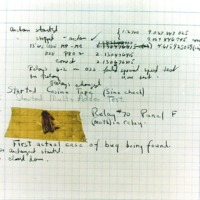
\includegraphics[width=3cm]{image/first-bug}
            \end{columns}
        \end{itemize}
    \end{frame}

    \begin{frame}{Qu'est-ce qu'un bug informatique~?}
        \begin{itemize}

            \item Bug dans les têtes, comme le bug de l'an 2000.
            Lié au format de date YY-MM-DD. Pas de gros soucis connus mais jusqu'à 80\% d'annonces d'embauche en plus dans les SSII françaises…
            \item Le pilote automatique Tesla, \textquote{Certain 2016-2023 Model S, Model X,2017-2023 Model 3, and 2020-2023 Model Y vehicles equipped with Full Self-Driving Beta (FSD Beta) software or pending installation}\footnote{Tesla, \url{https://www.tesla.com/en_eu/support/annual-and-recall-service}}
            \item Le pilote automatique du Boeing 737 MAX après 2 crashes, \textquote{Boeing agrees with the FAA's decision and request, and is working on the required software}\footnote{Boeing, conférence de presse, \url{https://theaircurrent.com/aviation-safety/faa-and-boeing-initially-disagreed-on-severity-of-catastrophic-737-max-software-glitch/}}
            \item WhatsApp et la vie privée, zero day RCE découvertes régulièrement, comme en 2022\footnote{Sophos, CVE-2022-36934 et CVE-2022-27492, integer overflow et underflow, \url{https://nakedsecurity.sophos.com/2022/09/27/whatsapp-zero-day-exploit-news-scare-what-you-need-to-know/}}
        \end{itemize}
    \end{frame}

    \begin{frame}{Qu'est-ce qu'un bug informatique~?}
        \begin{columns}
            \column{0.6\textwidth}
            Bug de 2038, le 19 janvier 2038 à 3 h 14 min 7 s soit le 1 janvier 1970 plus \lstinline{0b10**31}, i.e., 32bit en secondes
            \column{0.4\textwidth}
            \centering
            
\includegraphics[width=2cm]{image/bug-business}
        \end{columns}
        \begin{columns}
            \column{0.4\textwidth}
            \centering
            
\includegraphics[width=2cm]{image/hall-eye}
            \column{0.6\textwidth}
            Celui qui reste de la S.F., où l'humain perd le contrôle sur l'IA
        \end{columns}
        \begin{columns}
            \column{0.6\textwidth}
            Très divers mais le plus souvent, il est \textquote{entre la chaise et le clavier\ldots}
            \column{0.4\textwidth}
            \centering
            
\includegraphics[width=2cm]{image/working-together}
        \end{columns}

    \end{frame}

    \begin{frame}{Combien coûte un bug informatique~?}
        \begin{itemize}
            \item Plus il est trouvé tôt dans la vie du logiciel, moins il coûte.

            Donc, on teste le plus possible pour ne pas trouver de bug en production (e.g., recall, DeFi).

            C'est le \textquote{Shift left}~!
            \item En développement on paie le correctif, en production son impact
            \item Postulat du génie logiciel, c'est que le correctif est moins coûteux que l'impact
            \item Le coût de l'impact dépend du domaine, mais peut être très élevé, comme dans la DeFi, cf. \url{https://rekt.news/fr/}
        \end{itemize}
        \bigbreak
        \centering
        
\includegraphics[width=2cm]{image/milions-of-dolar-bills-burning}
    \end{frame}

    \begin{frame}{Capacités du génie logiciel moderne~?}
        \begin{itemize}
            \item Nous

            \item Les connaissances acquises dans ce module~:

            \begin{itemize}
                \item Bonnes pratiques de développement
                \item Testing automatique
                \item Bonnes pratiques de développement
                \item Outils collaboratifs de développement
                \item CI/CD, (CI = Continuous Integration (cf. Mise en place d'un serveur d'intégration continue), CD = Continous Delivery (cf. Déploiement de la version validée))
            \end{itemize}
        \end{itemize}
        \bigbreak
        \centering
        
\includegraphics[width=2cm]{image/programmer-shaking-hand-with-computer}
    \end{frame}


    \section{Bonnes pratiques}\label{sec:bonnes-pratiques}

    \begin{frame}{Bonnes pratiques, sommaire}
        \begin{itemize}
            \item Langages modernes comme Java et Python
        \end{itemize}
        \begin{columns}
            \column{0.6\textwidth}
            \begin{itemize}
                \item Parfois générales ou propres à une convention, un langage
                \item Les outils
                \item Pas de syntaxe \emoji{prohibited}
                \item Pas d'architecture \emoji{prohibited}
            \end{itemize}
            \column{0.4\textwidth}
            \centering
            
\includegraphics[width=4cm]{image/maniac-programmer-sorting-her-code}
        \end{columns}
    \end{frame}

    \begin{frame}{Bonnes pratiques, pourquoi?}
        \begin{itemize}
            \item Les nouvelles applications et les développements en cours et à venir
            \item Le correctif
            \item La maintenance évolutive
            \item Le code legacy, même si elles étaient moins formalisées, le bon sens a toujours existé~!
        \end{itemize}
    \end{frame}

    \begin{frame}{Bonnes pratiques, l'approche de Python}
        \begin{itemize}
            \item Python a une syntaxe éloignée des langages de son temps qui sont toutes déclinées de celle du C. Les syntaxes de C, C++, C\#, Java et même JavaScript
            \item Le pari d'une nouvelle syntaxe était risqué, mais G. Van Rossum souhaite une meilleure lisibilité
            \item \textquote{code is read much more often than it is written. The guidelines provided here are intended to improve the readability of code and make it consistent across the wide spectrum of Python code. As PEP 20 says, \textbf{Readability counts}}\footnote{Guido Van Rossum, \url{https://peps.python.org/pep-0008/}}
        \end{itemize}
    \end{frame}

    \begin{frame}[fragile]{Bonnes pratiques, l'approche de Python}
        \begin{lstlisting}
In [1]: import this
The Zen of Python, by Tim Peters

Beautiful is better than ugly.
Explicit is better than implicit.
Simple is better than complex.
Complex is better than complicated.
Flat is better than nested.
Sparse is better than dense.
Readability counts.
Special cases aren't special enough to break the rules.
Although practicality beats purity.
Errors should never pass silently.
Unless explicitly silenced.
In the face of ambiguity, refuse the temptation to guess.
There should be one-- and preferably only one --obvious way to do it.
Although that way may not be obvious at first unless you're Dutch.
Now is better than never.
Although never is often better than *right* now.
If the implementation is hard to explain, it's a bad idea.
If the implementation is easy to explain, it may be a good idea.
Namespaces are one honking great idea -- let's do more of those!
        \end{lstlisting}
    \end{frame}

    \begin{frame}[fragile]{Bonnes pratiques, l'approche de Python}
        En cas d'oubli, le mantra de Python A.K.A The Zen of Python, est dans l'interpréteur~!

        \bigbreak

        Le bon sens paysan fait consensus dans tous les langages de programmation~!

    \end{frame}

    \begin{frame}[fragile]{Bonnes pratiques, Python et PEP}
        \begin{columns}
            \column{0.5\textwidth}
            \begin{itemize}
                \item PEP est la convention de codage recommandée par Python, comme PEP8, le Style Guide for Python Code, à lire SVP
                \item Définit les espaces utiles à la lisibilité et les inutiles
                \item Snake\_case pour les variables
                \item Définit les casses et la déclaration~:
                \begin{itemize}
                    \item Attribut et méthode privé/publique~:
                \end{itemize}
            \end{itemize}
            \column{0.5\textwidth}
            \begin{lstlisting}[language=python]
class Case:
    public = 0

Case.public

Out[3]: 0

class Case:
    __private = 0

In [13]: Case.__private
---------------------------------------------------------------------------
AttributeError                            Traceback (most recent call last)
Cell In [13], line 1
----> 1 Case.__private

AttributeError: type object 'Case' has no attribute '__private'
            \end{lstlisting}
        \end{columns}
    \end{frame}

    \begin{frame}[fragile]{Bonnes pratiques, Python et PEP}
        \begin{itemize}
            \item Déclaration des constantes en upper case avec underscore, comme la plupart des langages~:
            \begin{lstlisting}[language=python]
In [17]: PLANCK_CONSTANT = 6.62607015*(10^-34) # Upper case with underscore for constants

In [18]: PLANCK_CONSTANT = 42 # But constant those not really exists in Python

In [19]: PLANCK_CONSTANT
Out[19]: 42
            \end{lstlisting}
            \item Déclaration des classes en CamelCase et fonctions en snake\_case~:
            \begin{lstlisting}[language=python]
In [20]: class UnNomEnCamelCase:
...:     pass
...:

In [21]: def un_verbe_au_moins_en_snake_case():
...:     pass
...:
            \end{lstlisting}
        \end{itemize}

    \end{frame}

    \begin{frame}[fragile]{Bonnes pratiques, Python et PEP}
        \begin{itemize}
            \item Les commentaires, en ligne si possible~:
            \begin{lstlisting}[language=python]
In [22]: is_even = lambda x: x % 2 == 0  # Il est clair que l'on commente cette ligne mais c'est long

In [23]: # Retourne True pour un chiffre pair

In [24]: is_even = lambda x: x % 2 == 0
            \end{lstlisting}
            \item Favoriser l'indentation même si la syntaxe en ligne est valide, après les \textquote{:} des conditions et des déclarations~:
            \begin{lstlisting}[language=python]
def is_even(x):return x % 2 == 0 # Pas biennnn

def is_even(x):
    return x % 2 == 0 # Biennnn
            \end{lstlisting}
        \end{itemize}

    \end{frame}

    \begin{frame}{Bonnes pratiques, l'IDE, une aide précieuse}
        \centering

        $\vcenterimage{image/Pycharm-before-analysis}\vcenterarrow\vcenterimage{image/Pycharm-after-analysis}$

        \bigbreak

        \begin{flushleft}
            Dans la fenêtre dédiée aux divers warnings et erreurs, après analyse du project, les IDEs modernes détaillent de multiples types d'erreurs et warnings.
            Ils peuvent même les corriger automatiquement.

            Une liste non exhaustive des IDEs ouverts~:
            \begin{itemize}
                \item VS Code (Avec Black formatter et Pylint)
                \item Pycharm pour Python
                \item Eclipse pour Java
                \item IntelliJ pour Java
                \item Zed (\url{https://zed.dev/}, sur Mac OS et Linux pour l'instant uniquement)
            \end{itemize}
        \end{flushleft}

    \end{frame}

    \begin{frame}{Bonnes pratiques, l'IDE, intégration à des outils tiers}

        \centering
        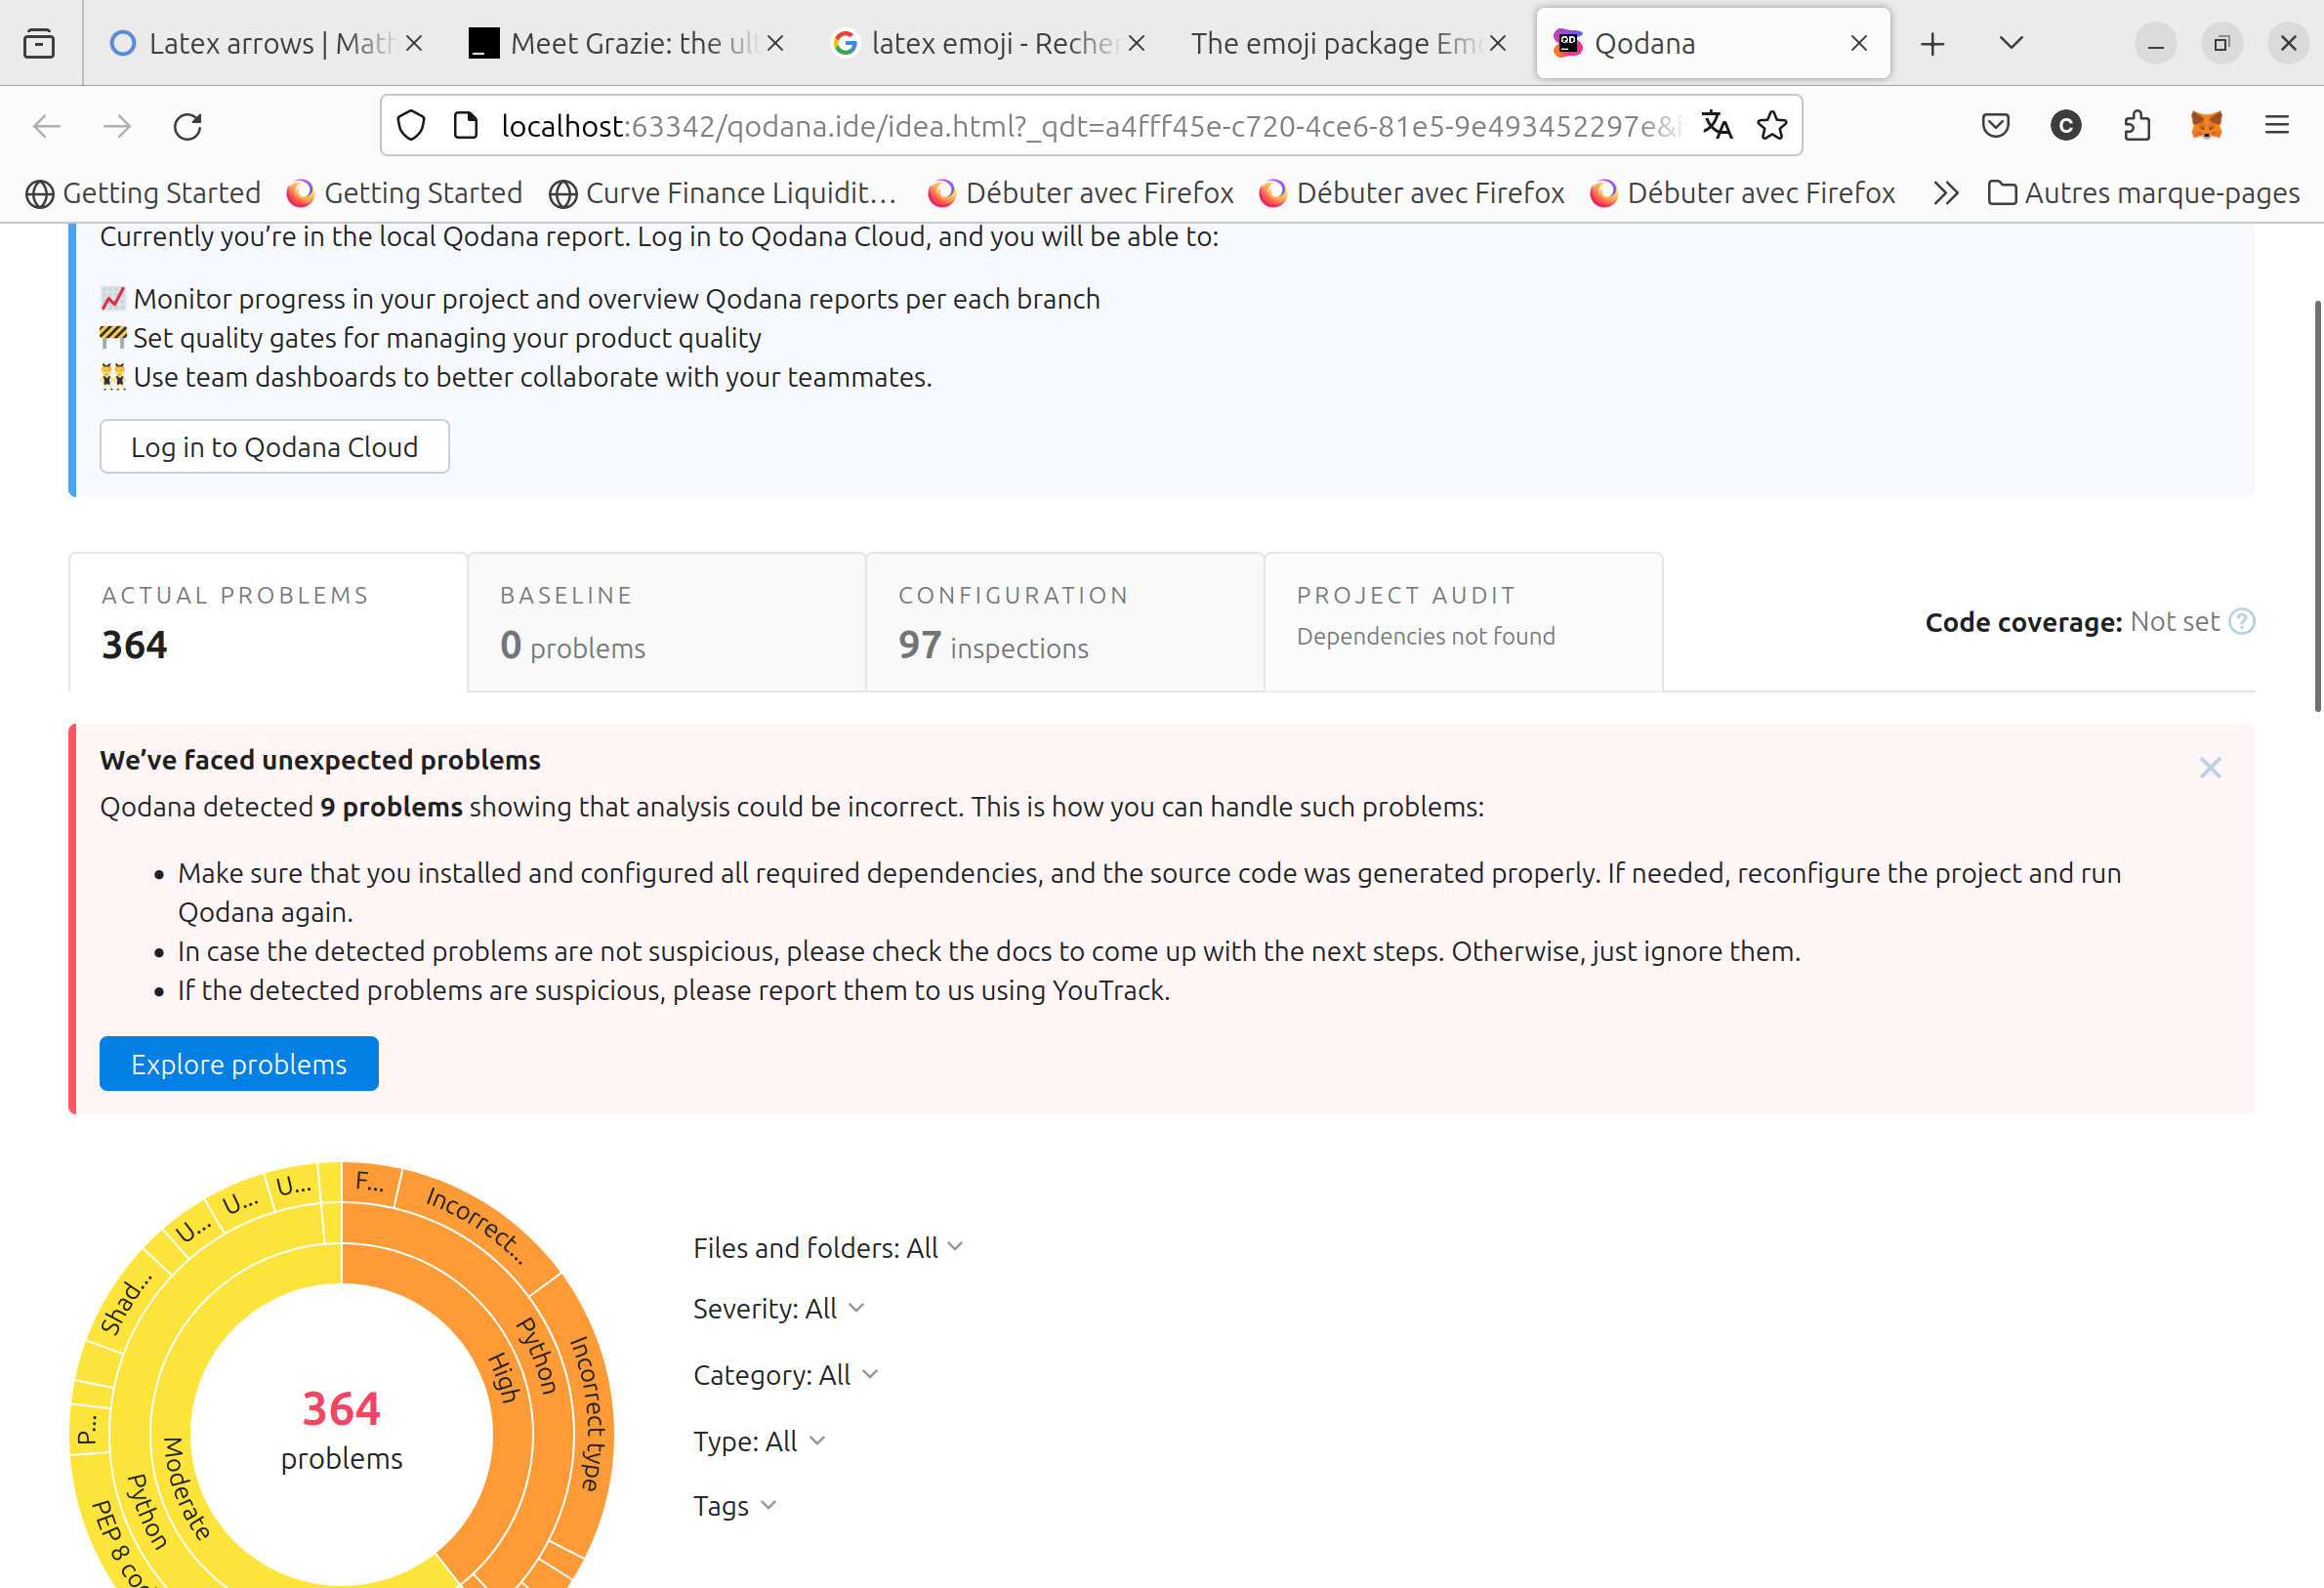
\includegraphics[width=5cm]{image/Qodana-result}

        \bigbreak

        \begin{flushleft}
            Certains plugins peuvent se connecter à des applications dédiées à l'analyse des sources comme SonarQube \emoji{flag-switzerland}, Qodana, etc.
            Ils permettent une analyse plus complète et d'enregistrer des indicateurs permettant de suivre l'évolution dans le temps de la qualité des sources du projet.
        \end{flushleft}
    \end{frame}

    \begin{frame}{Bonnes pratiques, l'IDE, lire les indications}

        \begin{itemize}
            \item VS Code ou Pycharm ont toutes ces fonctionnalités modernes
            \item Dans la carte, sur le côté on voit rapidement les soucis sur tout un fichier
            \bigbreak
            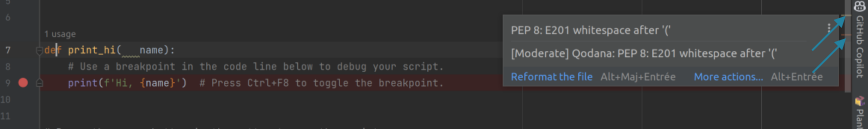
\includegraphics[width=8cm]{image/Pycharm-minimap}
            \item Dans le code source en cours d'édition
            \bigbreak
            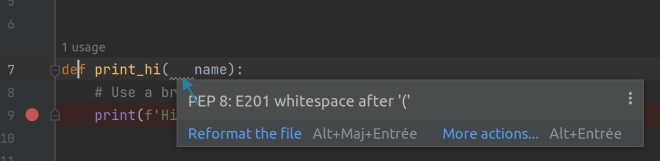
\includegraphics[width=8cm]{image/Pycharm-waring-in-code}
        \end{itemize}

    \end{frame}

    \begin{frame}{Bonnes pratiques, l'approche de Java}

        \begin{itemize}

            \item Développé au début des années 90 chez Sun Microsystems, racheté par Oracle, actuellement le principal développeur
            \item \textquote{Its syntax is similar to C and C++, but it omits many of the features that make C and C++ complex, confusing, and unsafe.}\footnote{Oracle, Java Virtual Machine Specification, \url{https://docs.oracle.com/javase/specs/jvms/se8/html/jvms-1.html}}
            \item Plus safe au niveau de la mémoire car il a un ramasse miette et plus simple à coder.
            Mais la syntaxe doit être familière pour les développeurs et donc s'inspirer des langages de l'époque C et C++

        \end{itemize}

    \end{frame}

    \begin{frame}{Bonnes pratiques, l'approche de Java}
        Oracle, Java code conventions\footnote{Oracle, Java code conventions, \url{https://www.oracle.com/java/technologies/javase/codeconventions-introduction.html}}~:
        \bigbreak

        \begin{itemize}

            \item 80\% of the lifetime cost of a piece of software goes to maintenance.
            \item Hardly any software is maintained for its whole life by the original author.
            \item Code conventions improve the readability of the software, allowing engineers to understand new code more quickly and thoroughly.
            \item If you ship your source code as a product, you need to make sure it is as well packaged and clean as any other product you create.

        \end{itemize}

    \end{frame}

    \begin{frame}{Bonnes pratiques, l'approche de Java du nommage}

        Oracle, Java naming convention (identique pour JavaScript)\footnote{Oracle, Java code conventions, \url{https://www.oracle.com/java/technologies/javase/codeconventions-namingconventions.html}}~:
        \bigbreak

        \centering
        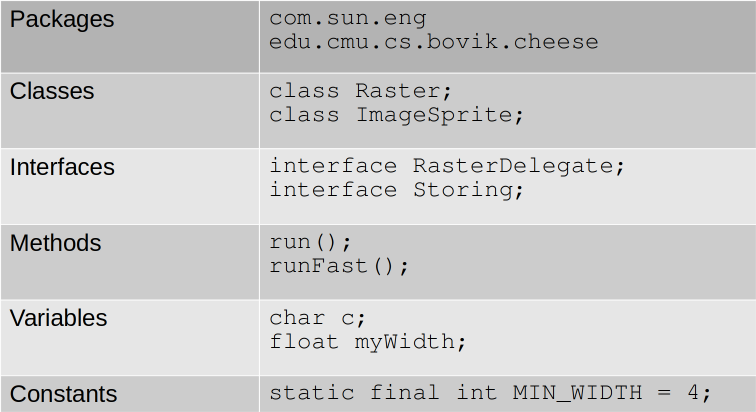
\includegraphics[width=8cm]{image/Java-naming-convention}

    \end{frame}

    \begin{frame}[fragile]{Bonnes pratiques, ne pas abuser des fonctionnalités du typage dynamique}
        \pause
        Les attribues d'un objet peuvent être définis dynamiquement mais cela empêche d'explorer la structure d'un objet lors du développement~:
        \begin{lstlisting}[language=python]
class DynamiqueMaisPasTrop:
    def __init__(self):
        self.bien = 0 # bien sera toujours visible dans l'IDE
    def a_appeler(self):
        self.pas_bien = 0 # Ne sera pas visible avant l'exécution de a_appeler
        \end{lstlisting}

        Tous les IDE seront perdus et l'attribue \lstinline{pas_bien} ne sera pas visible avant l'exécution de la fonction \lstinline{a_appeler}, comme ici IPython~:

        \centering
        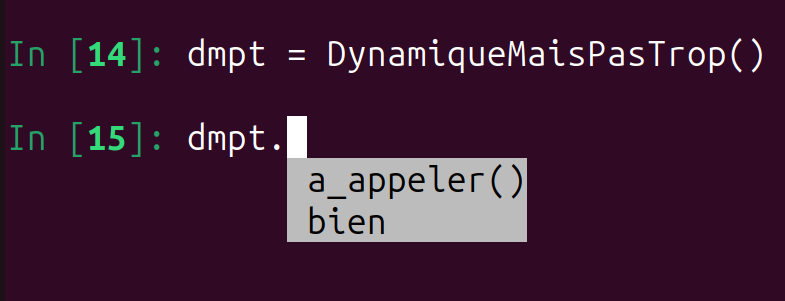
\includegraphics[width=5cm]{image/dynamic-trick}

        \begin{flushleft}
            Tous les attribues doivent être définis dans le constructeur.
            PEP le recommande en Python par exemple.
            Cf. l'exemple à ne pas suivre d'SQLAlchemy
        \end{flushleft}

    \end{frame}


    \begin{frame}{Bonnes pratiques, les différences entre Java et Python}

        \begin{itemize}

            \item Rien à voir avec Python
            \item Java est typé statiquement, Python dynamiquement
            \item Majoritairement du CamelCase
            \item Pas du tout de snake\_case
            \item Majoritairement du CamelCase
            \item Pas du tout de snake\_case
            \item Toutes les JVM ont une compatibilité ascendante~!
            \item Quand Python a une nouvelle bonne idée, elle peut être intégrée, on verra plus tard la compatibilité\ldots e.g., la célèbre rupture de compatibilité Python 2 à 3

        \end{itemize}

        \centering
        
\includegraphics[width=8cm]{image/Java-vs-Python}

    \end{frame}

    \begin{frame}[fragile]{Bonnes pratiques, les flottants et leurs pièges}
        \pause
        Peu de nombres réels peuvent être représentés avec exactitude en informatique~\footnote{Floating Point Arithmetic: Issues and Limitations, \url{https://docs.python.org/3/tutorial/floatingpoint.html}}\textsuperscript{,}\footnote{What Every Computer Scientist Should Know About Floating-Point Arithmetic, \url{https://docs.oracle.com/cd/E19957-01/806-3568/ncg_goldberg.html}}:

        \begin{lstlisting}[language=python]
In [8]: 0.2 + 0.1 == 0.3 # Should be True
Out[8]: False

In [9]: 2/10 + 1/10 == 3/10 # Should be True
Out[9]: False

In [10]: 1/2 + 4/16 + 1/16 == 8/16 + 4/16 +1/16 # Should be True
Out[10]: True
        \end{lstlisting}

        De l'arithmétique simple peut donc être fausse~!
    \end{frame}

    \begin{frame}[fragile]{Bonnes pratiques, les flottants et leurs pièges}

        Les réels sont exacts s'ils peuvent être représentés par une fraction sous la forme~:\[ x / 2^y \]

        Sinon, le nombre réel est représenté par la fraction la plus approchante.

        Python a une méthode d'introspection des flottants~:

        \begin{lstlisting}[language=python]
In [15]: from math import log, isclose

In [16]: (1/3).as_integer_ratio()
Out[16]: (6004799503160661, 18014398509481984)

In [17]: numerateur, denominateur = (0.3333333333333333333333333333333333333).as
    ...: _integer_ratio() # Le numerateur est 6004799503160661

In [18]: log(denominateur, 2)
Out[18]: 54.0
In [18]: isclose(1/3, numerateur / 2**54)  # True if the closest fraction
Out[18]: True
        \end{lstlisting}

        La fraction la plus proche du flottant de valeur 1/3 est~:\[ 6004799503160661 / 2^{54} \]

    \end{frame}

    \begin{frame}[fragile]{Bonnes pratiques, les flottants et leurs pièges et leurs solutions}

        \begin{columns}
            \column{0.7\textwidth}
            Une des solutions, est de toujours utiliser des entiers quand c'est possible!

            Pour des devises, utiliser des entiers pour les centimes.
            Voir même faire tous les calculs en centimes et ne convertir en euros par exemple, qu'à l'affichage.
            \column{0.3\textwidth}
            \centering
            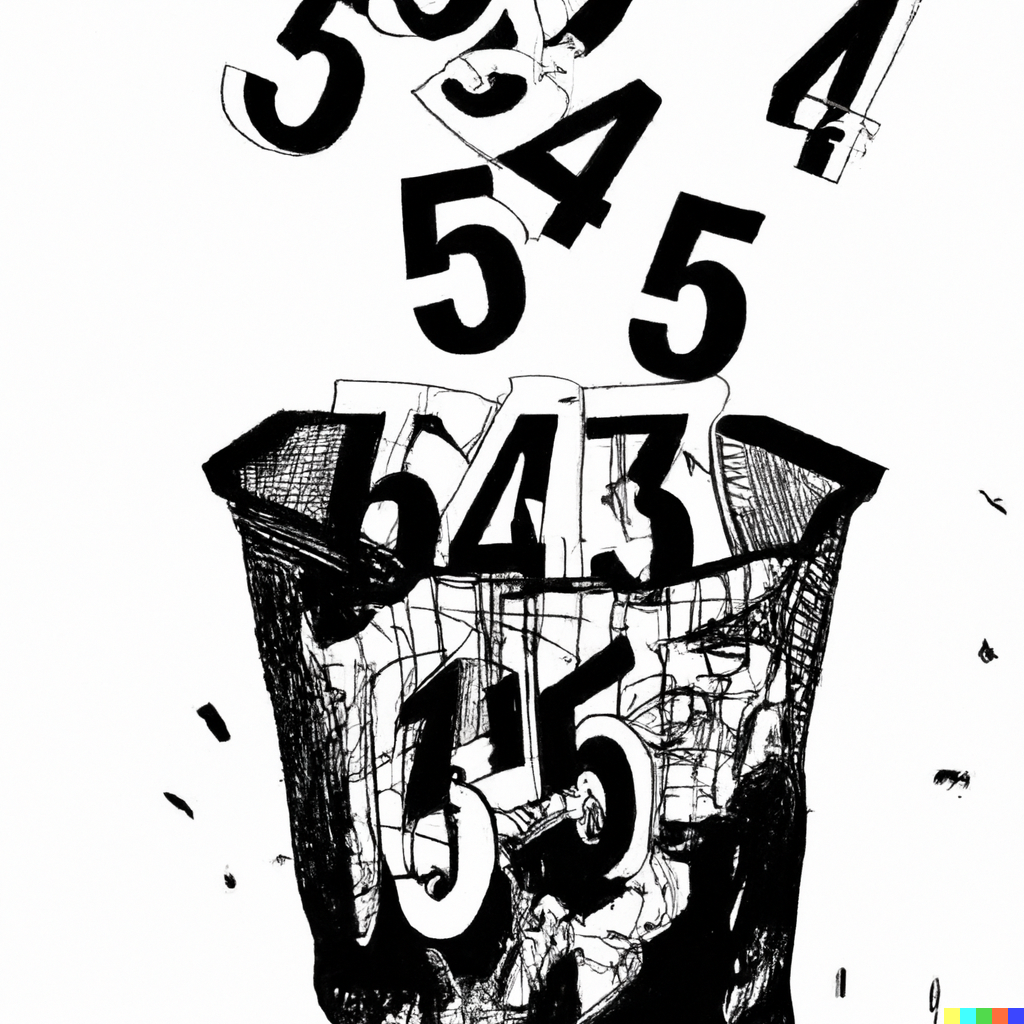
\includegraphics[width=3cm]{image/numbers-throwned-in-the-trash}

        \end{columns}
        \begin{lstlisting}[language=python]
class EuroCents: # Des centimes et de l'arithmétique sans flottant !
    def __init__(self, cents):
        self.cents = cents
    def __repr__(self):
        return str(self.cents / 100) + " €"
    def __add__(self, val):
        return EuroCents(self.cents + val.cents)

montant = EuroCents(5) + EuroCents(5)
print(montant) # >>> 0.1 €
        \end{lstlisting}

        Sinon, utiliser des librairies avec des types et fonctions dédiées aux nombres réels.
    \end{frame}

    \begin{frame}{Bonnes pratiques, les autres langages}

        \begin{itemize}

            \item JavaScript n'a pas de coding style officiel publié par l'ECMA International
            \item Certaines sociétés ou communautés ont publié des coding styles populaires~:

            \begin{itemize}
                \item Google JavaScript Style Guide
                \item Airbnb JavaScript Style Guide
                \item JavaScript Standard Style (n'a de standard que le nom)
                \item Idiomatic
            \end{itemize}
            \item PHP a PSR, c'est l'acronyme PHP Standard Recommendation
            \item Pour tout langage, suivre la convention officiel ou une mainstream

        \end{itemize}

    \end{frame}

    \begin{frame}{Bonnes pratiques, pour tous}
        \begin{columns}
            \column{0.6\textwidth}
            \begin{itemize}

                \item Certaines pratiques issues du bon sens et de l'expérience dans le développement logiciel s'appliquent à tous les langages.
                C'est plus essentiel que de connaître la dernière architecture logiciel à la mode
                \item Un best seller, la bible, d'où viennent certaines bonnes pratiques de ce cours, Clean Code: A Handbook of Agile Software Craftsmanship par Robert C. Martin
                \item Ou CODER PROPREMENT par Robert C. Martin\ldots

            \end{itemize}
            \column{0.4\textwidth}
            \centering
            
\includegraphics[width=3cm]{image/kid-reading}
        \end{columns}

    \end{frame}

    \begin{frame}{Bonnes pratiques, pour tous}
        The Total Cost of Owning a Mess\footnote{Robert C. Martin, Clean Code: A Handbook of Agile Software Craftsmanship}~:
        \bigbreak
        \centering
        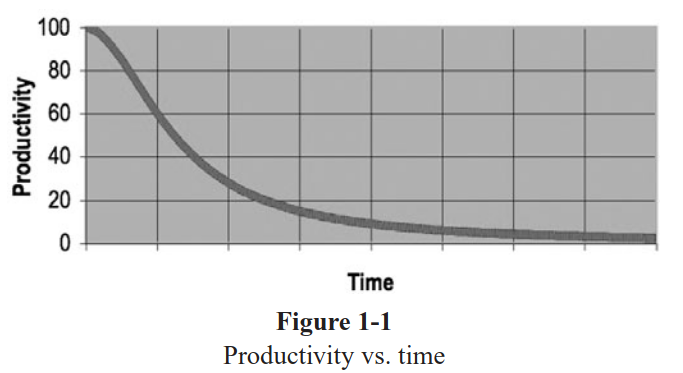
\includegraphics[width=10cm]{image/total-cost-of-a-mess}
    \end{frame}

    \begin{frame}{Bonnes pratiques, le fichier source pour tous}
        \begin{itemize}

            \item Une ligne fait 80 caractères de long maximum si possible (Java, Python, Clean Code)
            \item Penser aux vertical rulers des IDE, à 80, 100, 120 caractères par exemple
            \item Héritage de la carte perforée mais surtout pour faire rentrer facilement la ligne dans un écran/terminal
            \item Indenter tout, les déclarations de classe ou de fonction, les conditions même quand le langage ne l'oblige pas comme Java

        \end{itemize}
    \end{frame}

    \begin{frame}{Bonnes pratiques, le fichier source pour tous}

        Créer des fichiers sources par classe ou fonction, avec un nombre de lignes le plus réduit possible.

        \bigbreak
        \centering
        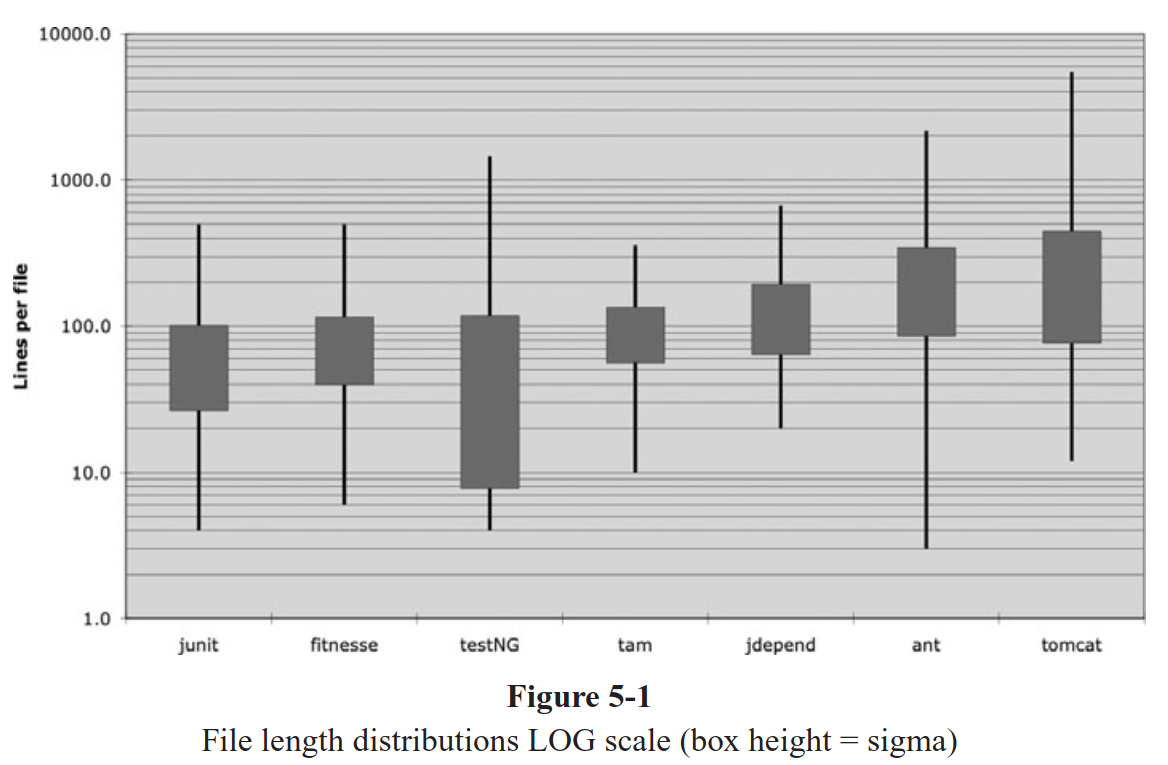
\includegraphics[width=10cm]{image/project-source-length}

    \end{frame}

    \begin{frame}{Bonnes pratiques, le fichier source pour tous}

        \begin{columns}
            \column{0.5\textwidth}
            \centering
            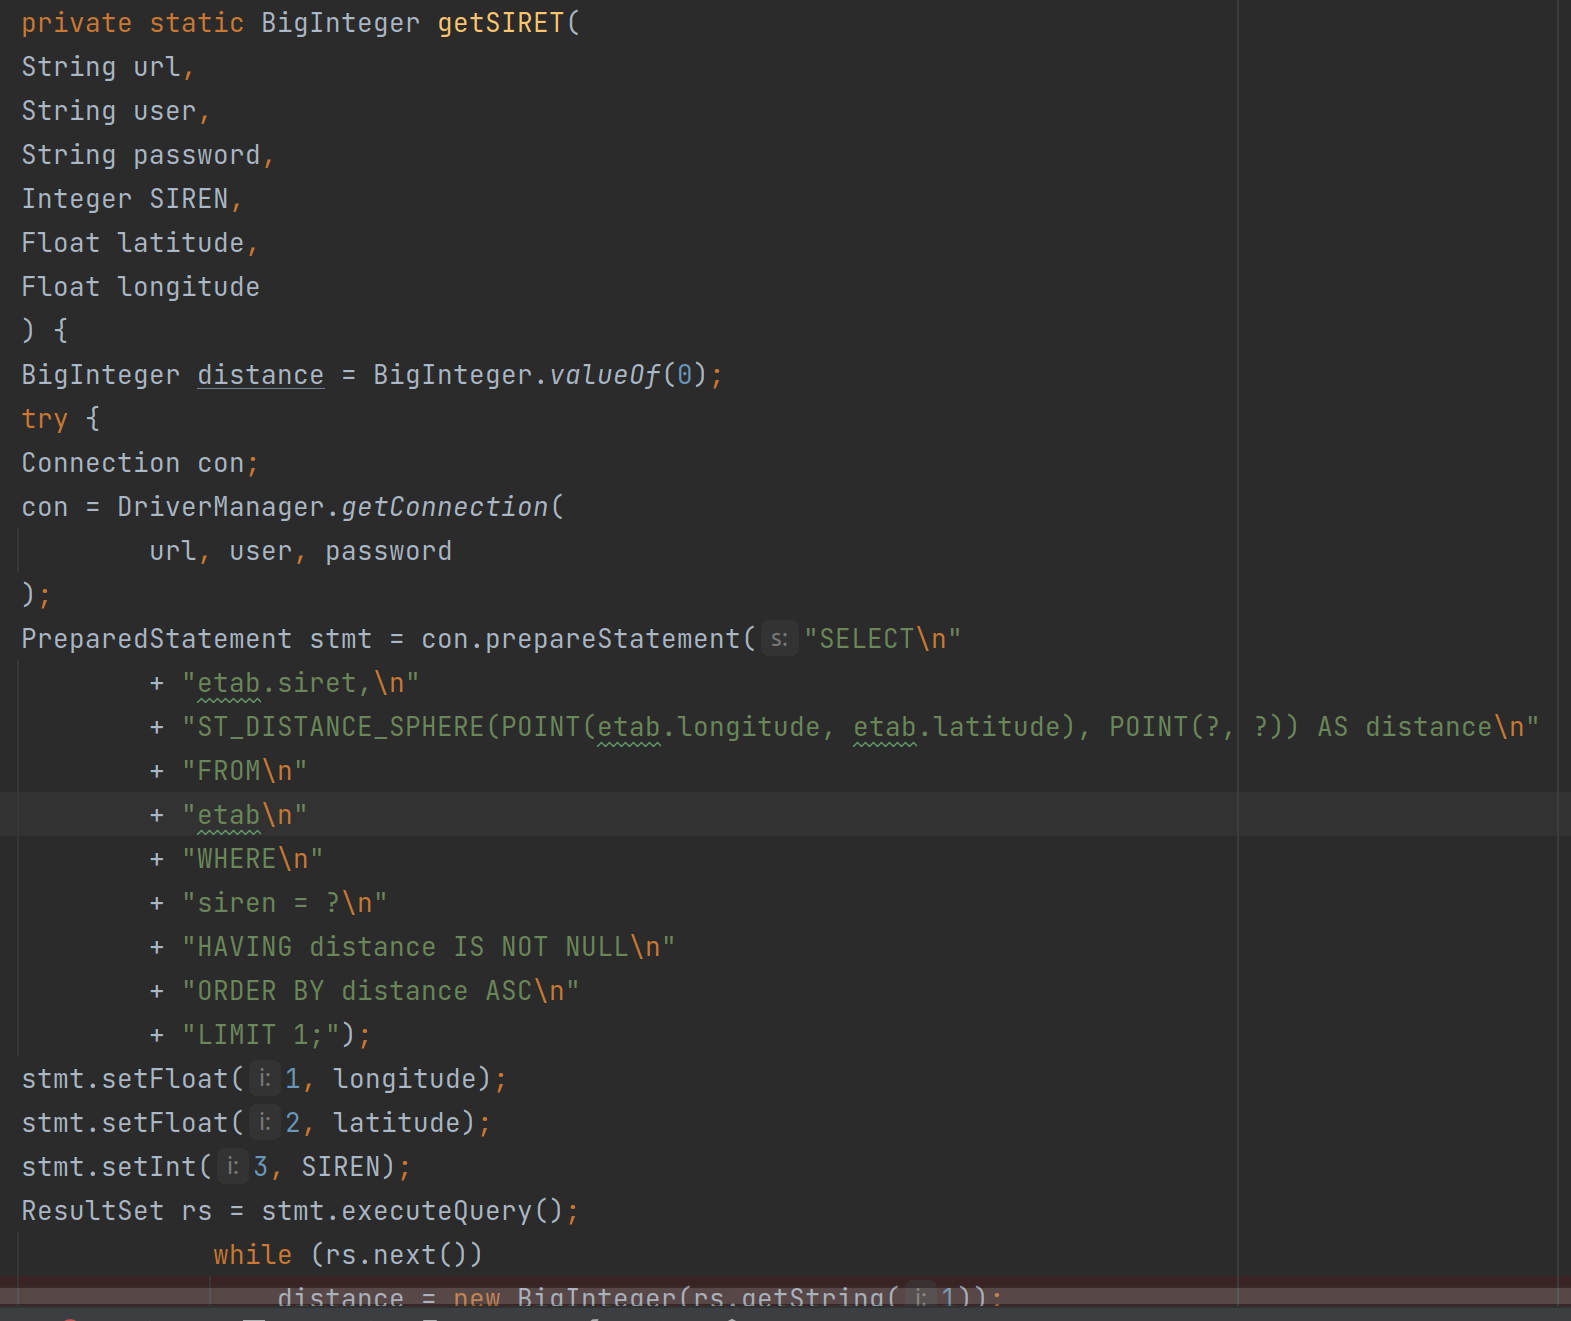
\includegraphics[width=5cm]{image/numerous-identations}
            \column{0.5\textwidth}
            \centering
            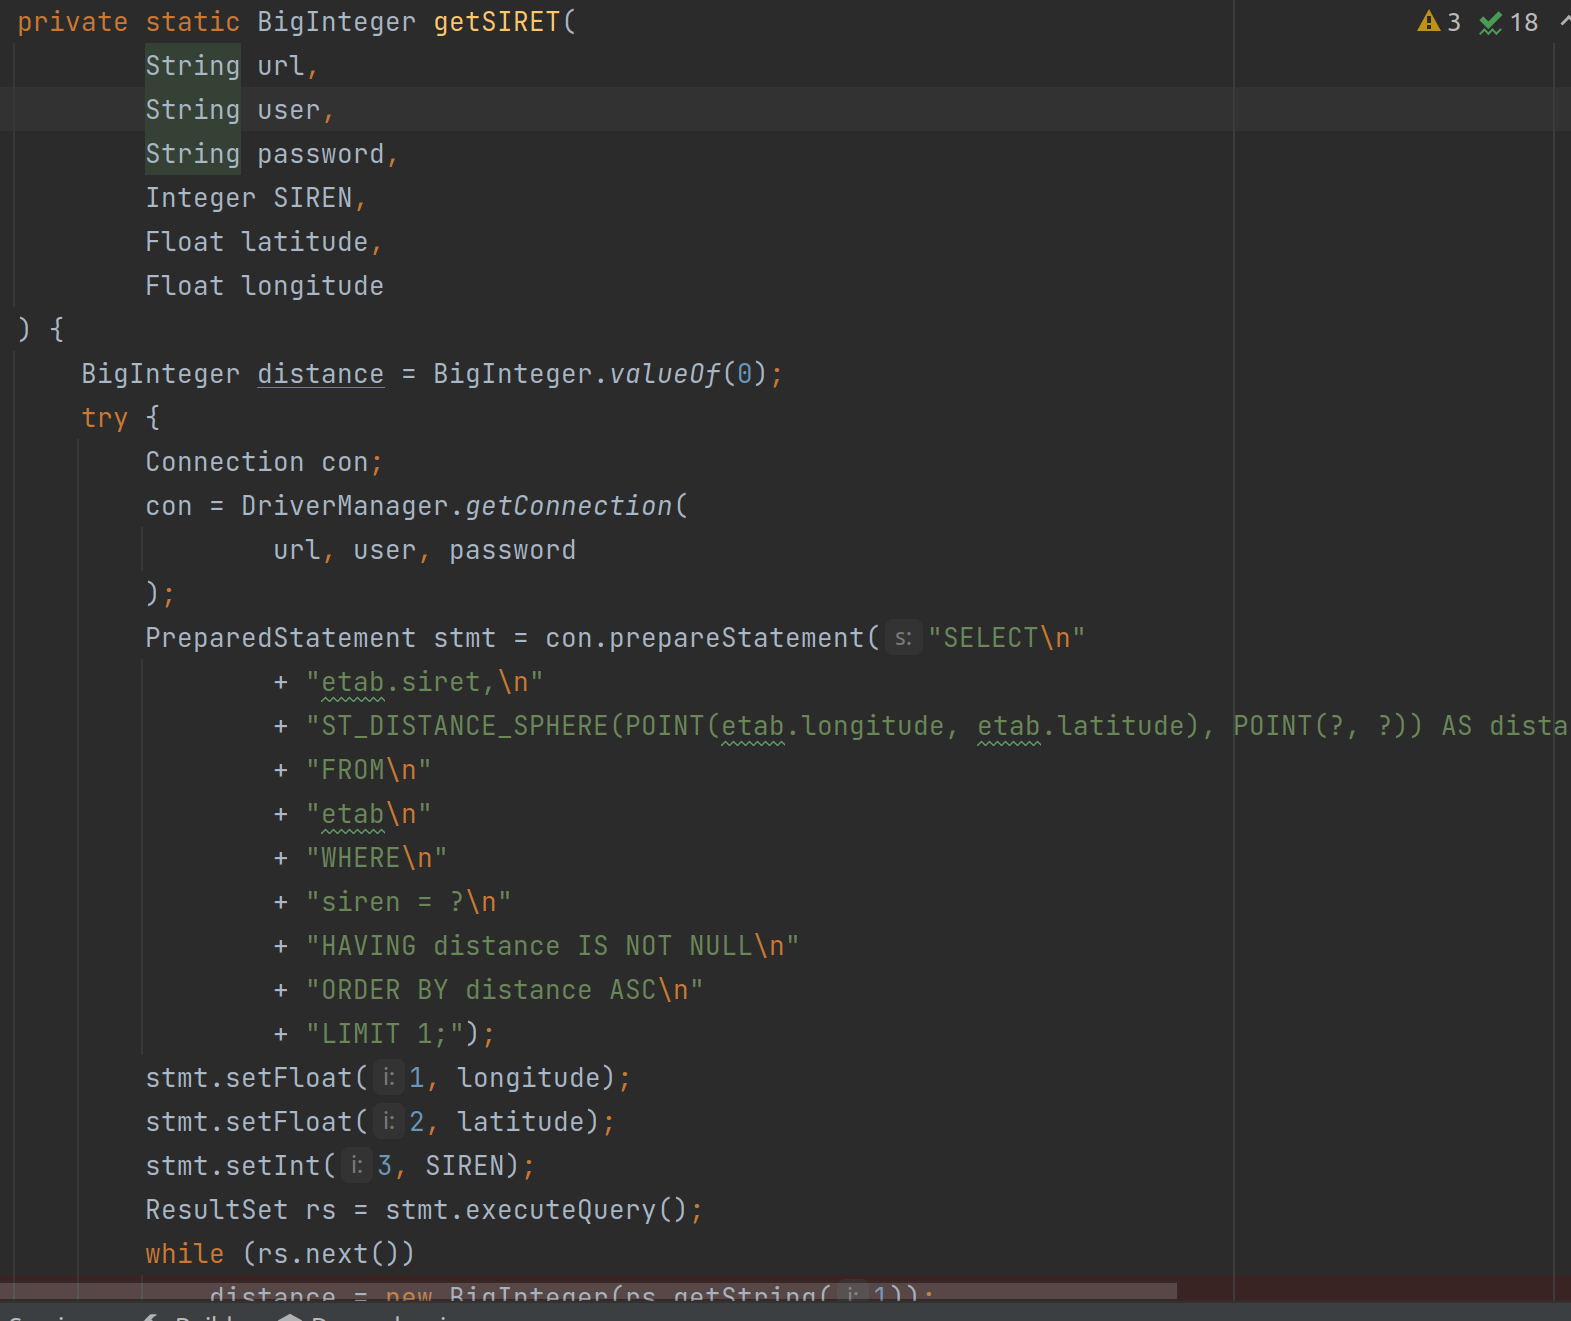
\includegraphics[width=5cm]{image/one-identation}
        \end{columns}

    \end{frame}

    \begin{frame}{Bonnes pratiques, le naming pour tous}

        \begin{itemize}

            \item Donner aux variables des noms qui ont du sens
            \item Des noms qui doivent révéler vos intentions
            \item Correcte dans la langue dans laquelle vous développez
            \item Prononçable
            \item Que l'on peut rechercher dans les sources, pas de variable d'1, 2, 3 lettres

        \end{itemize}
        \bigbreak

        \quad\texttt{int d; // elapsed time in days }\quad\emoji{pouting-face}
        \bigbreak
        \quad\texttt{int elapsedTimeInDays; }\quad\emoji{two-hearts}
    \end{frame}

    \begin{frame}{Bonnes pratiques, le naming pour tous}

        \begin{itemize}

            \item Éviter la désinformation
            \item L'information sur le type doit être précise et exacte
            \item Pas de L, de I ni de O

        \end{itemize}
        \bigbreak

        \quad\texttt{Queue<Integer> ageList; }\quad\emoji{pouting-face}
        \bigbreak
        \quad\texttt{Queue<Integer> ages; }\quad\emoji{two-hearts}
    \end{frame}

    \begin{frame}{Bonnes pratiques, le naming pour tous}

        \begin{itemize}

            \item Une variable instance de classe est un nom et un ou plusieurs qualificatifs différenciant cette instance
            \item Les noms des méthodes et fonctions contiennent au moins un verbe sinon une phrase succincte donc avec verbe également
            \item Simple à mémoriser
            \item Un mot seul par concept.
            Par exemple en anglais retourner une value pourrait utiliser~:
            \begin{itemize}
                \item Return
                \item Fetch
                \item Get
                \item Retrieve
                \item …
            \end{itemize}
            \item Ne pas dupliquer d'information en répétant un contexte déjà présent dans les niveaux supérieurs.
            E.g., dans un package dont le nom est celui de la compagnie il est inutile de répéter ce nom dans les classes

        \end{itemize}
    \end{frame}

    \begin{frame}{Bonnes pratiques, les fonctions pour tous}

        \begin{itemize}

            \item Une bonne fonction est petite
            \item La plus petite possible
            \item Doit avoir la responsabilité d'une seule action, celle décrite dans son nom
            \item Pure ou avec effet secondaire mais pas les deux
            \item S'inspirer de la programmation fonctionnelle pour créer des fonctions pures le plus atomique possible

        \end{itemize}
    \end{frame}

    \begin{frame}{Bonnes pratiques, les fonctions pour tous}

        \centering
        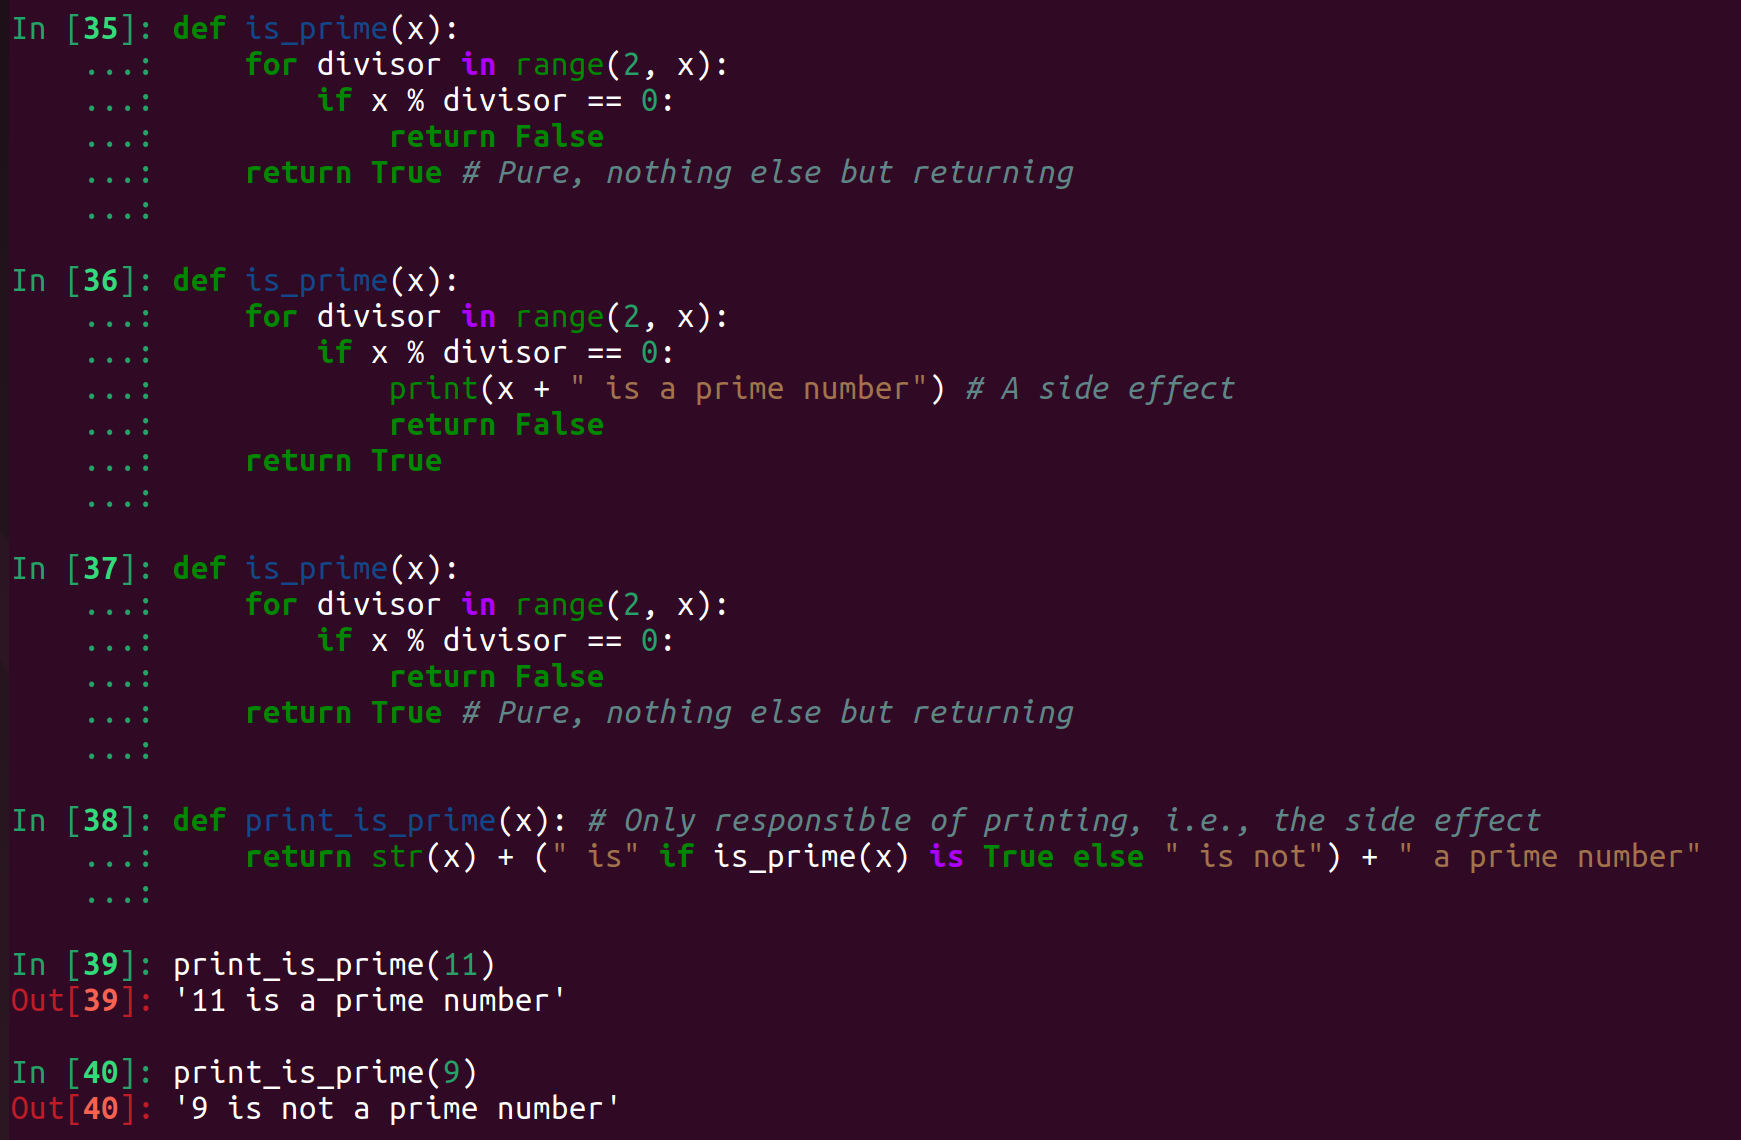
\includegraphics[width=10cm]{image/pure-se-functions}
    \end{frame}

    \begin{frame}{Bonnes pratiques, les fonctions pour tous}
        \begin{itemize}

            \item Atomique, i.e., les fonctions ne font qu'une chose
            \item Si vous avez plusieurs sections ou plusieurs commentaires, c'est un signe que votre fonction fait plus qu'une chose
            \item Si possible un seul argument, éventuellement 2, maximum 3
            \item Pour réduire à un argument, pensez à transformer un ensemble d'arguments en classe avec ses attribues pour un langage OO, ou une struct (C, Rust), variable groupée (CoBOL)

        \end{itemize}
    \end{frame}

    \begin{frame}{Bonnes pratiques, les fonctions pour tous}
        Les IDE modernes ont le plus souvent une fonction pour créer automatiquement une fonction (e.g., intelliJ)
        \centering
        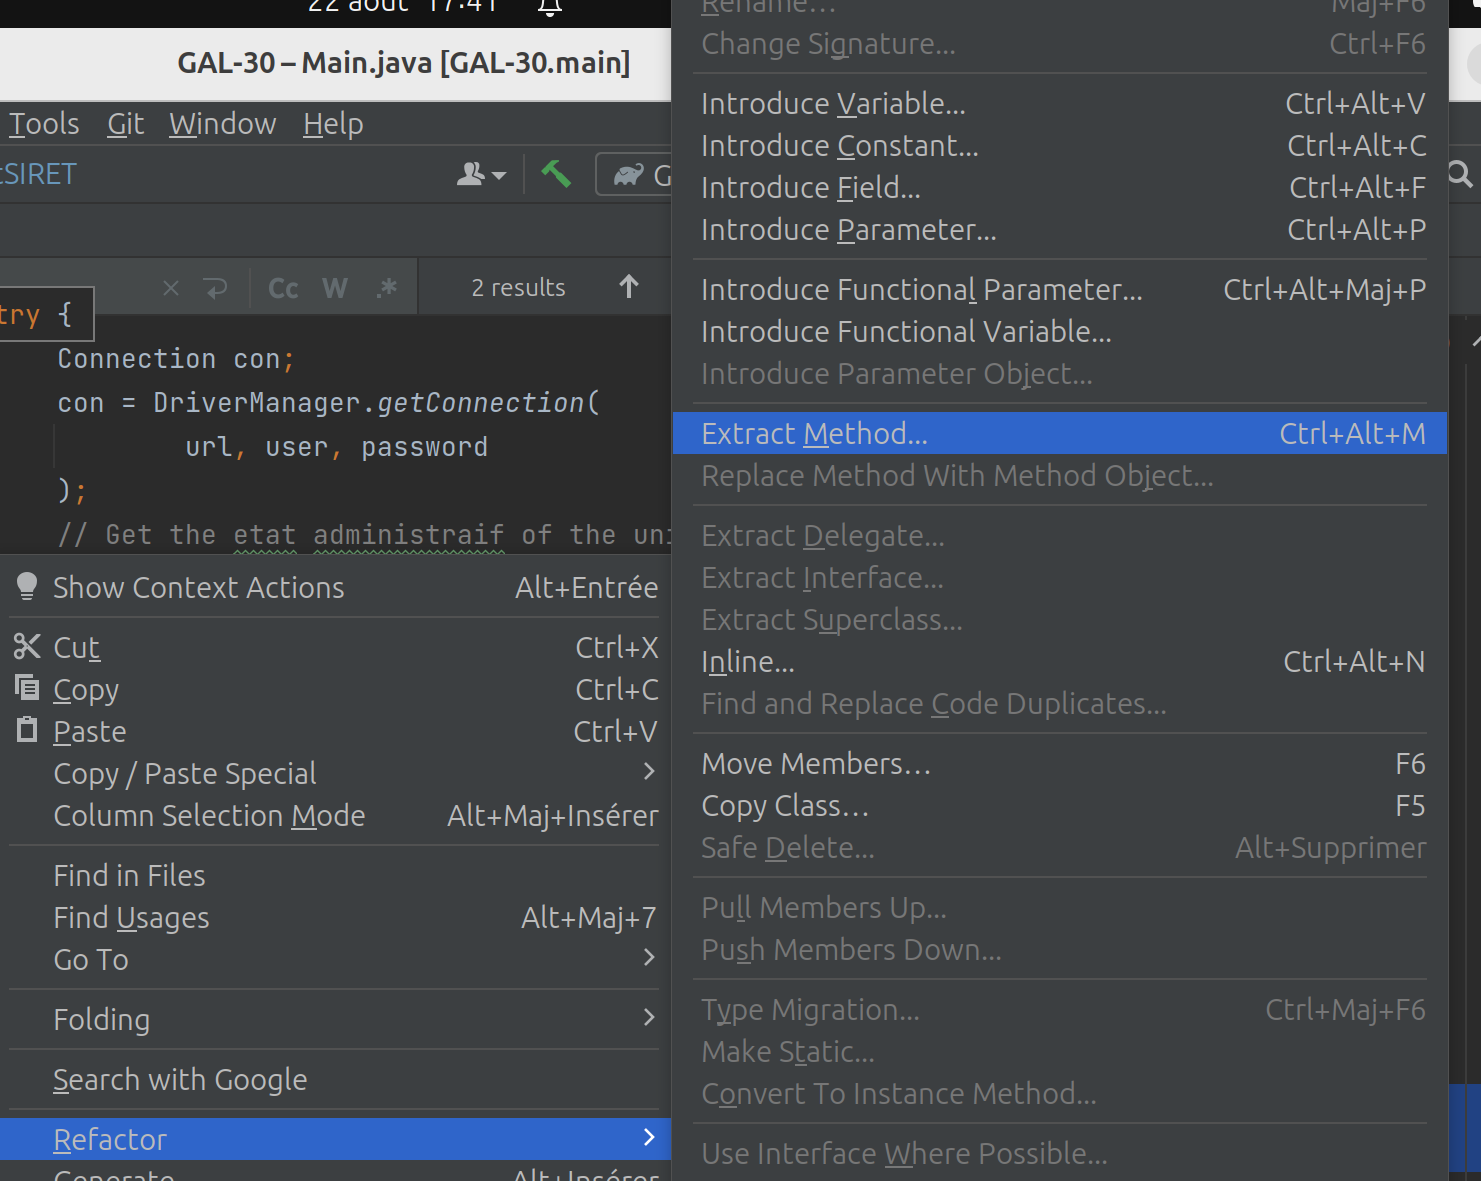
\includegraphics[width=10cm]{image/ide-gen-function}
    \end{frame}

    \begin{frame}{Bonnes pratiques, les fonctions pour tous}
        \begin{columns}
            \column{0.5\textwidth}
            \begin{itemize}

                \item Pas de modification de l'argument passé par référence
                \item La fonction a une action sur le(s) argument(s) et donne une valeur de sortie à retourner
                \item A droite, l'argument passé \lstinline{outer\_list} est modifié mais cela se comprend difficilement
                \item En plus, cela dépend du type de l'argument passé en Java comme en Python, voir ci-dessous

            \end{itemize}
            \column{0.5\textwidth}
            \centering
            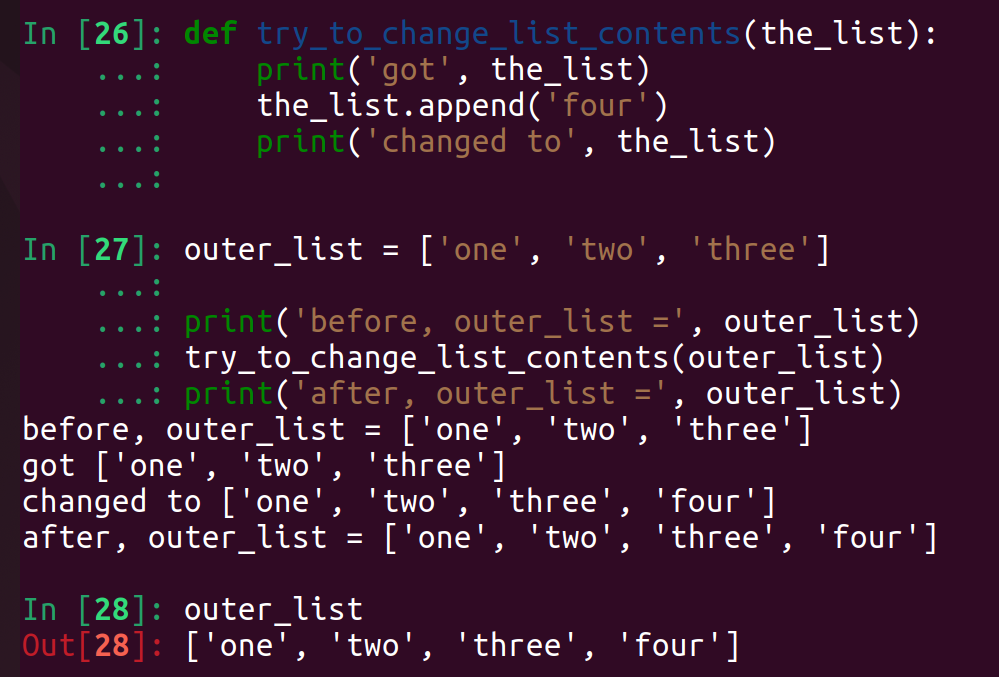
\includegraphics[width=5cm]{image/arg-modified-by-reference}
            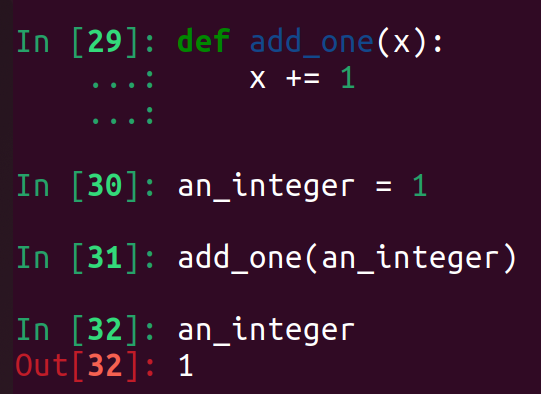
\includegraphics[width=5cm]{image/arg-not-modified}
        \end{columns}
    \end{frame}

    \begin{frame}{Bonnes pratiques, les fonctions pour tous}
        \begin{columns}

            \column{0.4\textwidth}
            \centering
            
\includegraphics[width=5cm]{image/doing-many-things}

            \column{0.6\textwidth}
            \begin{itemize}

                \item Command Query Separation, A.K.A CQRS (Command and Query Responsibility Segregation), une fonction à action sur une base de donnée, API, c'est une Command.
                Quand on requête une donnée en base ou dans une API c'est une Query
                \item Cela permet également d'avoir une fonction avec moins de responsabilités

            \end{itemize}

        \end{columns}
    \end{frame}

    \begin{frame}[fragile]{Bonnes pratiques, les commentaires pour tous}


        \begin{itemize}

            \item Sont un complément aux commentaires structurés de l'autodocumentation comme Sphinx ou Javadoc (cf. la suite du cours)
            \item Sur la même ligne si cela ne fait pas une ligne trop longue
            \item Expliquer ses intentions
            \item Commentaires spéciaux comme les TODO (reste à faire) et NoQA (à tester) sont très utiles
            \item Ne pas commenter du code, le VCS est là pour créer l'historique du code
            \item Ne jamais partir du principe que les autres vont lire le commentaire et se contenter d'expliquer les problèmes à éviter dans les commentaires.
            C'est trop dangereux, il faut corriger l'algorithme

        \end{itemize}
        \begin{lstlisting}[language=python]
# En cas de plantage ne pas relancer ce script, en cas de plantage dans la fonct
# ion update_the_balance, cela envoie l'argent 2 fois dans la fonction
# send_the_money
import .send_the_money, .update_the_balance
send_the_money()
update_the_balance()
        \end{lstlisting}
    \end{frame}

    \begin{frame}{Bonnes pratiques, les classes pour l'OOP, héritage ou composition}

        \centering
        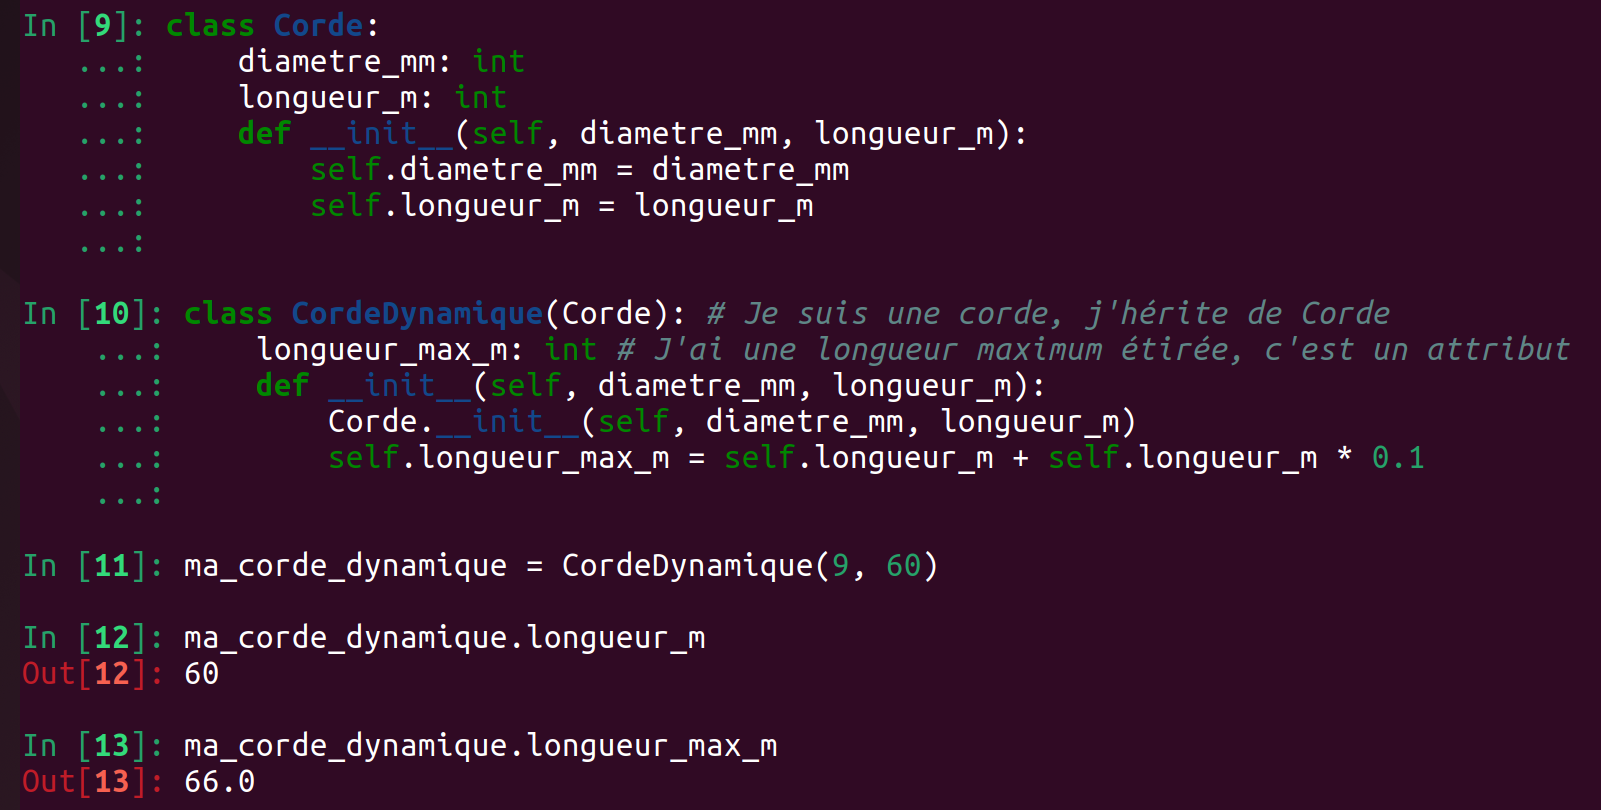
\includegraphics[width=10cm]{image/inheritance-or-composition}

    \end{frame}

    \begin{frame}{Bonnes pratiques, les classes pour l'OOP}

        L'héritage évite les if/else et switch/case

        \centering

        $\vcenterimage{image/if-else}\vcenterarrow\vcenterimage{image/inheritance-bird}$

    \end{frame}

    \begin{frame}{Autres livres sur les bonnes pratiques}

        \begin{itemize}

            \item Steven C. McConnell, Code Complete Second Edition
        \end{itemize}
        \bigbreak

        \centering
        
\includegraphics[width=5cm]{image/an-inifinity-of-books}

    \end{frame}

    \begin{frame}{Génération de la documentation, les frameworks d'autodocumentation}

        \begin{itemize}

            \item Pourquoi ne pas documenter un programme dans un simple fichier Word~?
            \item L'autodocumentation ajoute à un document de base (e.g., le README) la description du code présente dans des commentaires structurés du fichier source
            \item Des frameworks propres à un langage, d'autres pour tous les langages et chacun ou presque a son modèle de commentaires structurés
            \item Ceux pour tous les langages ont l'avantage de ne s'apprendre qu'une fois sinon on en apprend un pour chaque langage
            \item Celui spécifique à un langage aura plus de chance d'être connu des développeurs de la communauté
            \item Les officiels, à préférer et les autres issues de plus petites communautés
        \end{itemize}

    \end{frame}

    \begin{frame}{Génération de la documentation, Java et Javadoc}

        \begin{itemize}

            \item Autodocumentation officielle des sources Java
            \item Chaque déclaration de classe ou fonction Java a un commentaire avec des tags du langage de balisage Javadoc
            \item Spécification Javadoc \url{https://www.oracle.com/fr/technical-resources/articles/java/javadoc-tool.html}
        \end{itemize}
        \bigbreak

        \centering
        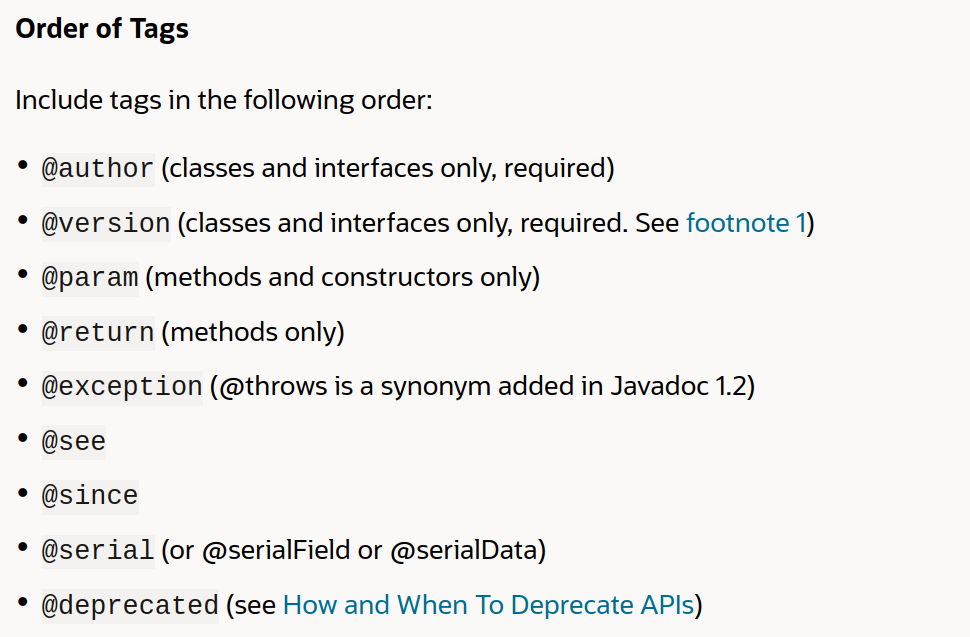
\includegraphics[width=5cm]{image/javadoc-tags}
    \end{frame}

    \begin{frame}{Génération de la documentation, Javadoc avec un l'IDE,  IntelliJ}

        \centering
        $\vcenterimage{image/javadoc-example}\vcenterarrow\vcenterimage{image/javadoc}$
        \bigbreak

        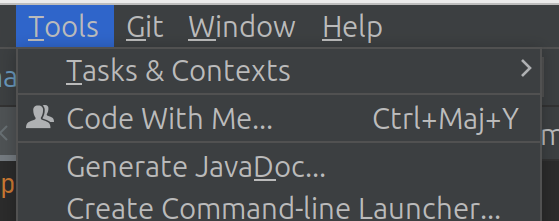
\includegraphics[width=5cm]{image/generate-button}

    \end{frame}

    \begin{frame}[fragile]{Génération de la documentation, Sphinx documentation avec PyCharm}

        \begin{itemize}

            \item Langage de balisage est ReStructured Text, similaire au markdown mais différent (dommage\ldots). Formatage très complet, permet de faire des UI riches.
            Voir \url{https://www.sphinx-doc.org/en/master/usage/restructuredtext/index.html} pour la définition
            \item Le README peut-être ajouté avant les commentaires du code.
            Il doit être au format RST (README.rst), Markdown (README.md), word, etc
            \item L'avantage des README Markdown et RST est qu'ils sont mis en forme par les serveurs comme GitHub, Gitlab\ldots
            \item Toutes les documentations sont dans les docstrings, une structure propre à Python.
            Les docstrings sont dans l'attribue \lstinline{__doc__} qui peut être appelé dans le shell Python avec la fonction \lstinline{help}
            \item Documente les déclarations \lstinline{def} et \lstinline{class}
            \item Documente les modules avant le code

        \end{itemize}

    \end{frame}

    \begin{frame}{Génération de la documentation, Sphinx documentation avec PyCharm}

        \centering
        $\vcenterimage{image/python-rst}\vcenterarrow\vcenterimage{image/readme-example}$

    \end{frame}

    \begin{frame}{Génération de la documentation, Python et Sphinx documentation}
        README plus commentaires en RST des modules et des déclarations.

        \centering
        $\vcenterimage{image/python-rst-2}\vcenterarrow\vcenterimage{image/readme-plus-code}$

    \end{frame}

    \begin{frame}{Génération de la documentation, Python et Sphinx documentation}
        \begin{columns}
            \column{0.5\textwidth}
            Fonction Sphinx Doc intégrée dans PyCharm pour la génération de la documentation.
            \column{0.5\textwidth}
            \centering
            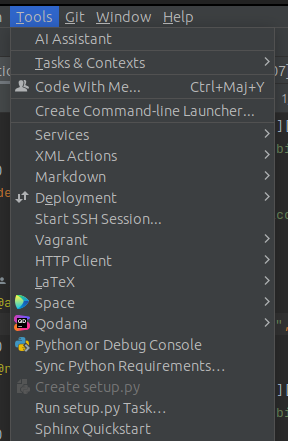
\includegraphics[width=4cm]{image/sphinx-generate-button}
        \end{columns}
    \end{frame}

    \begin{frame}{Génération de la documentation, Doxygen pour tous les sources}

        \begin{itemize}

            \item \textquote{Generate documentation from source code}, c'est aussi générique que cela! \emoji{smiling-face-with-halo}
            \item La liste des langages supportés est très longue, \textquote{C++, C, Objective-C, C\#, PHP, Java, Python, IDL, Fortran, and to some extent D}
            \item Comme JavaDoc, des tags sont rajoutés dans les commentaires
            \item Peut fonctionner avec les tags JavaDoc si configuré pour

        \end{itemize}
        \bigbreak

        \centering
        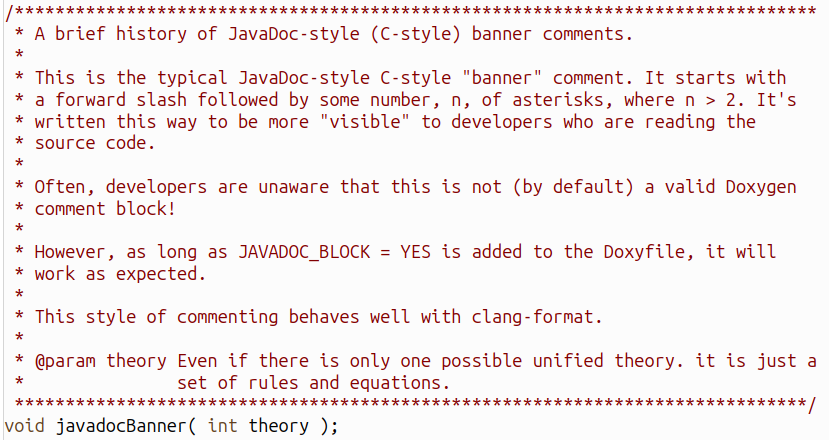
\includegraphics[width=7cm]{image/javadoc-with-doxygen}

    \end{frame}

    \begin{frame}{Génération de la documentation, Doxygen pour tous les sources}
        \begin{columns}

            \column{0.6\textwidth}
            \begin{itemize}

                \item Configurable comme tous les frameworks d'autodocumentation~:

                \begin{itemize}
                    \item Template
                    \item Type de document généré
                    \item Logo
                    \item …
                \end{itemize}
                \item En ligne de commande avec la commande doxygen \lstinline{doxygen -g <config-file>}

                \item Dans un GUI, le Doxygen wizard
                \item Cf. \url{https://www.doxygen.nl/}

            \end{itemize}

            \column{0.4\textwidth}

            \centering
            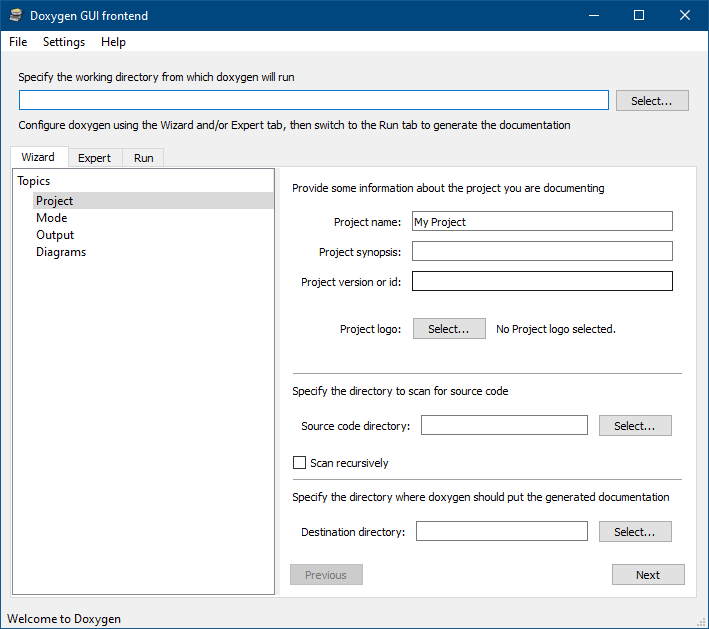
\includegraphics[width=5cm]{image/doxygen-configuration-hmi}

        \end{columns}

    \end{frame}

    \begin{frame}{Organisation du code d'un projet}

        \begin{itemize}

            \item Dépend du langage
            \item Dépend parfois du framework en plus
            \item Séparer les différents types de codes sources~:
            \begin{itemize}
                \item Code source de l'application
                \item Tests du code source
                \item Documentation
                \item CI/CD
            \end{itemize}
            \item Séparer les sources des dépendances externes
            \item Séparer les sources des fichiers générés (par la compilation, etc)
            \item Les fichiers temporaires et générés sont souvent dans un dossier caché (commençant par un point) pour être plus discret
            \item Pas toujours maîtrisable avec les dépendances~:
            \begin{itemize}
                \item Node JS, dans le \lstinline{node\_modules} du projet ou ailleurs en fonction de l'installation
                \item Dans le répertoire de l'interpréteur pour Python
                \item Dans un n'importe quel répertoire quand il n'y a pas de package manager comme en C/C++
            \end{itemize}

        \end{itemize}


    \end{frame}

    \begin{frame}{Organisation du code d'un projet, e.g., Java « classique » et Gradle }

        \begin{columns}

            \column{0.6\textwidth}
            \begin{itemize}

                \item Tout est séparé
                \begin{itemize}
                    \item Les ressources statiques
                    \item Les sources
                    \item Les tests
                    \item Le code compilé en classes
                    \item Le code compilé en exécutable JAR
                    \item La configuration de Gradle (Gère les dépendance, les builds, etc)
                    \item La documentation
                \end{itemize}
                \item Ce n'est qu'un exemple, une possibilité

            \end{itemize}

            \column{0.4\textwidth}

            \centering
            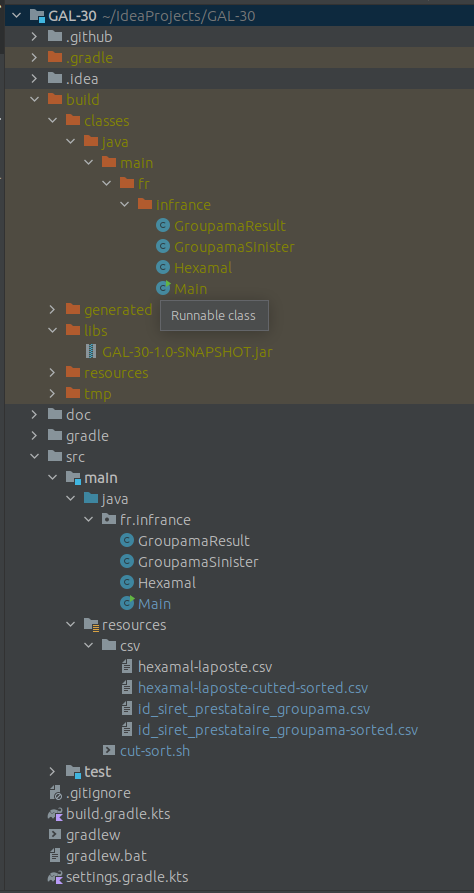
\includegraphics[width=4cm]{image/java-gradle-project-structure}

        \end{columns}

    \end{frame}

    \begin{frame}{Organisation du code d'un projet, e.g., Java Android et Gradle}

        \begin{columns}

            \column{0.6\textwidth}

            \centering
            
\includegraphics[width=2cm]{image/android-coffee}

            \begin{itemize}

                \item Tout est toujours séparé
                \item Différent du projet Java classique
                \item Des fichiers de configuration propres au développement Android
                \item Des fichiers de configuration propres au déploiement sur Playstore
                \item Ça dépend du projet, du framework, du déploiement, etc

            \end{itemize}

            \column{0.4\textwidth}

            \centering
            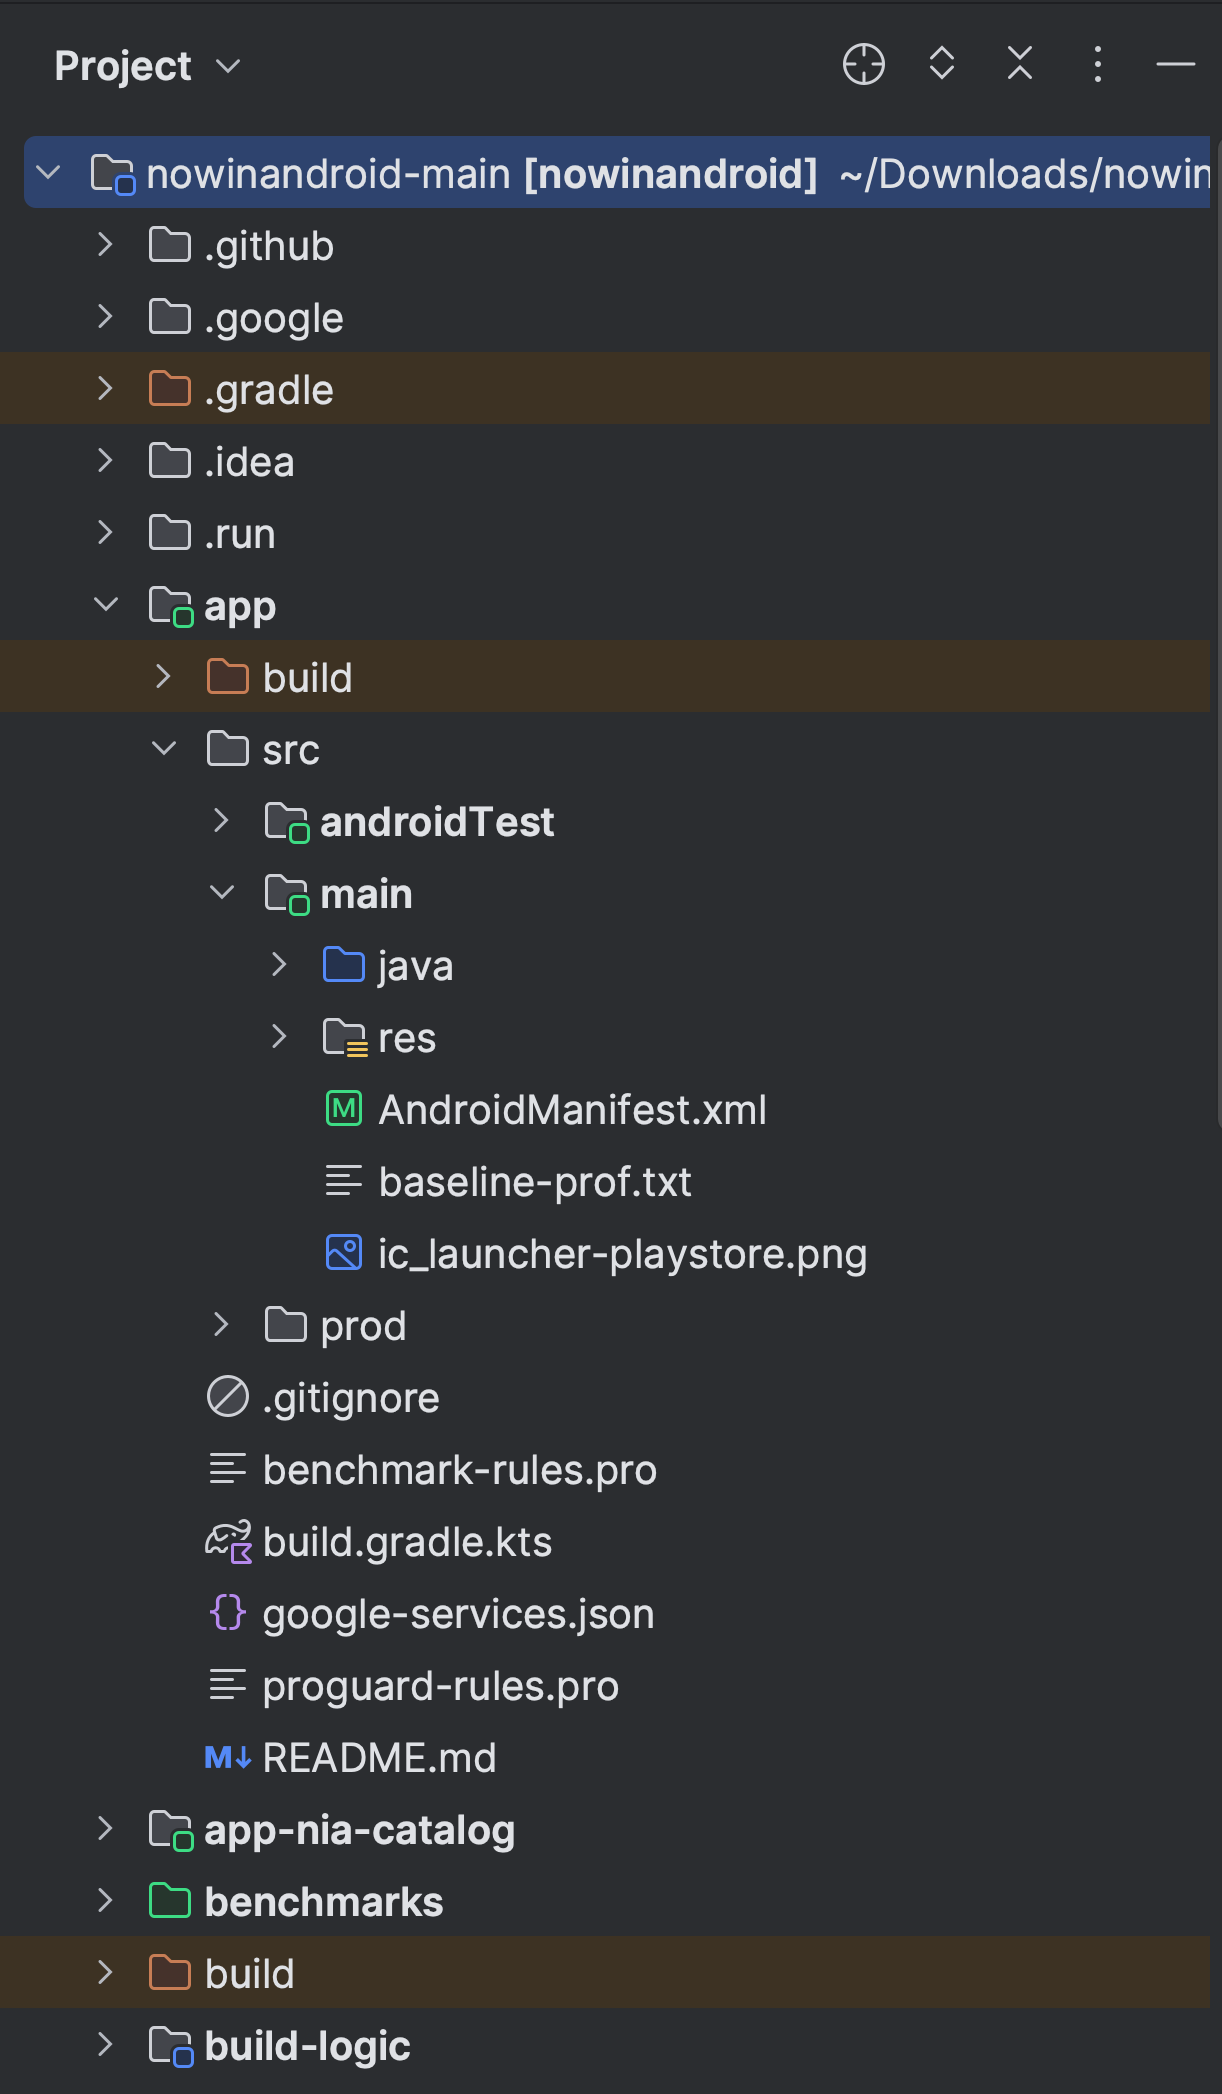
\includegraphics[width=4cm]{image/android-gradle-project-structure}

        \end{columns}

    \end{frame}

    \begin{frame}{Organisation du code d'un projet, Python, Solidity\ldots}

        \begin{columns}

            \column{0.6\textwidth}

            \begin{itemize}

                \item Framework style MVC avec tout dedans
                \item Exemple d'application \url{https://docs.djangoproject.com/en/4.2/intro/tutorial03}
                \item Le nom des dossiers et fichiers réfèrent explicitement à la fonction du source

            \end{itemize}

            \column{0.4\textwidth}

            \centering
            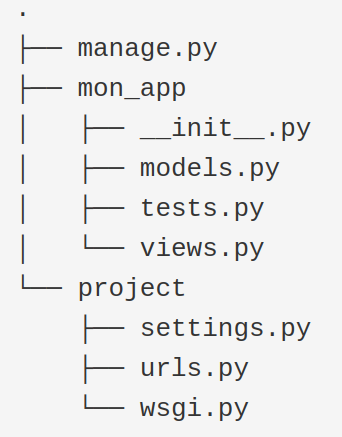
\includegraphics[width=3cm]{image/flask-project-structure}

        \end{columns}

        \begin{columns}

            \column{0.4\textwidth}

            \centering
            
\includegraphics[width=3cm]{image/smart-contract}

            \column{0.6\textwidth}
            \begin{itemize}

                \item Solidity est le langage de la Machine Virtual Ethereum (A.K.A EVM)
                \item L'environnement de développement de base RemixIDE ne support pas les imports
                \item Tout est donc dans un seul source, à comparer une fois compilé au bytecode présent dans la blockchain (voir Etherscan, CoinGecko)

            \end{itemize}


        \end{columns}

    \end{frame}

    \begin{frame}{Organisation du code d'un projet, Conclusion}

        \begin{itemize}

            \item L'organisation diffère entre les technos et même dans un même langage
            \item Différence entre les technos compilées et interprétées
            \item La bonne pratique, commune dans toutes les technos est le naming des dossiers et fichiers qui explicite la fonction du source
            \item Explorer les documentations et ressources officielles de chaque techno pour la bonne pratique en vigueur (RTFM encore une fois)

        \end{itemize}

        \centering
        
\includegraphics[width=3cm]{image/girl-reading-doc}

    \end{frame}

    \begin{frame}{Travaux dirigés, les sujets possibles}

        \begin{columns}
            \column{0.6\textwidth}
            \begin{itemize}

                \item Mettre en pratique tous les concepts vu dans ce cours
                \item Par groupe de 3 maximum
                \item Publier les résultats dans un repository sur plateforme comme Github, Gitlab
                \item Envoyer l'adresse du repository à \url{christophe.brun@papit.fr}

            \end{itemize}

            \column{0.4\textwidth}
            \centering
            
\includegraphics[width=4cm]{image/working-together}
        \end{columns}

        \begin{itemize}

            \item Mettre au propre votre projet perso
            \item Créer un soft inexistant simple.
            Par exemple comme ajouter des SRI inplace~:
            \begin{itemize}
                \item En Java
                \item En C++
            \end{itemize}
            \item Un projet open source déjà existant ne mettant pas en application les bonnes pratiques de ce cours.
            Raymond Hettinger a commencé par compléter des commentaires et la documentation de Python et conseille de faire de même pour être onboarder sur un projet OS
            \item Bien d'autres possibilités encore~!

        \end{itemize}

    \end{frame}


    \section{Tests unitaires}\label{sec:tests-unitaires}

    \begin{frame}{L'histoire du testing}

        \begin{itemize}

            \item ISTQB, l'International Software Testing Qualifications Board a été fondée en 1998\footnote{ISTQB, About Us, \url{https://www.istqb.org/about-us/who-we-are}}
            \item Dans son livre Extreme Programming Explained, Kent Beck parle de Test-first Programming en 1999
            \item Les standards modernes datent de la fin des années 90, début des années 2000
            \item JUnit, le framework de test le plus utilisé en Java date de 2002\footnote{Steven J Zeil, Unit Testing Frameworks, \url{https://www.cs.odu.edu/~zeil/cs350/latest/Public/junit/index.html}}
            \item Début du BDD (Behavior-Driven Development) avec JBehave, censé remplacer JUnit en utilisant le behavior au lieu de test, date de 2003\footnote{Cucumber, \url{https://cucumber.io/docs/bdd/history/}}
        \end{itemize}

    \end{frame}

    \begin{frame}{Qu’est-ce qu’un test~?}{Définition de l'International Software Testing Qualifications Board et IBM}
        \transdissolve
        L’ISTQB défini les termes suivants dans son glossaire\footnote{ISTQB, Glossaire des termes utilisés en tests de logiciels, \url{https://www.cftl.fr/wp-content/uploads/2018/10/Glossaire-des-tests-logiciels-v3_2F-ISTQB-CFTL-1.pdf}}~:

        \textbf{Test~:} Un ensemble d’un ou plusieurs cas
        de tests.

        \textbf{Cas de test~:} Un ensemble de conditions
        préalables, de données d'entrée, d'actions
        (le cas échéant), de résultats attendus et
        de postconditions, élaboré sur la base des
        conditions de test.
        \bigbreak
        Selon IBM\footnote{IBM, Qu'est-ce que le test logiciel~?, \url{https://www.ibm.com/fr-fr/topics/software-testing}}~:

        \textquote{Le test logiciel est le processus qui consiste à évaluer et à vérifier qu'un produit ou une application logicielle fait ce qu'il ou elle est censé(e) faire.}
    \end{frame}

    \begin{frame}{Qu’est-ce qu’un test unitaire~?}{Définition de la taverne du testeur\footnote{Mais c’est quoi un test unitaire~?, \url{https://latavernedutesteur.fr/2018/04/11/mais-cest-quoi-un-test-unitaire/}}}
        \transdissolve
        Il obéit au principe \textquote{F.I.R.S.T.}~:
        \begin{itemize}
            \item \textbf{Fast~:} S’exécute rapidement et est donc automatisé
            \item \textbf{Isolated~:} Est indépendant des facteurs externes et des autres tests
            \item \textbf{Repeatable~:} Isole les bugs automatiquement
            \item \textbf{Self-validating (autonome)~:} N’est pas ambiguë (pas sujet à interprétation, ne demande pas une action manuelle pour vérifier le résultat)
            \item \textbf{Timely (tôt)~:} Écrit en même temps que le code (même avant en TDD)
        \end{itemize}
        Si le test échappe à un de ces principes, il n'est probablement pas unitaire.
        \bigbreak
        Pour isoler les bugs automatiquement, un test unitaire doit tester le code unitairement, et isolement.
        Il doit donc être écrit dans le but de tester la logique d’une ligne de code, et quasiment si un test unitaire échoue vous pouvez connaitre la ligne de code incriminée.
    \end{frame}

    \begin{frame}{Testing, les frameworks de test unitaire}
        \begin{itemize}
            \item UnitTest, le framework de test standard de Python
            \item PyTest, un framework pour tout faire en Python
            \item JUnit, le framework de test le plus utilisé en Java
            \item PHPUnit, le framework de test standard de PHP
            \item Google Test, pour le C++
            \item Jest pour JS, Babel, pour TypeScript, Node, React, Angular, Vue et plus encore
            \item etc
        \end{itemize}
    \end{frame}

    \begin{frame}{La Pyramide des tests}
        \begin{columns}
            \column{0.3\textwidth}
            Différents types de tests peuvent être identifiés.
            La classification la plus classique étant la suivante\footnotemark~:
            \column{0.7\textwidth}
            \centering
            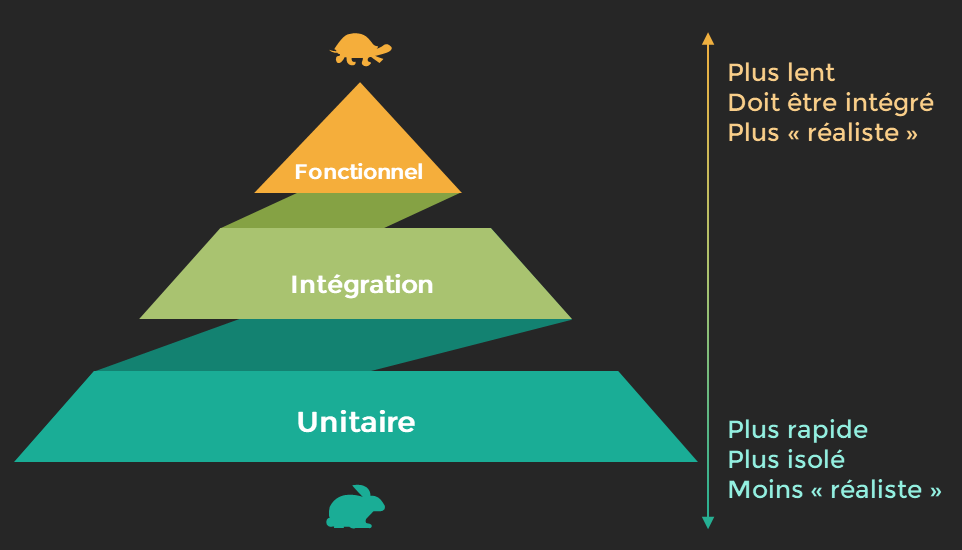
\includegraphics[width=7cm]{image/classic-test-pyramid}
        \end{columns}
        \bigbreak
        \footnotetext{OPENCLASSROOMS, Testez votre code Java pour réaliser des applications de qualité, \url{https://openclassrooms.com/fr/courses/6100311-testez-votre-code-java-pour-realiser-des-applications-de-qualite/6616481-decouvrez-les-tests-dintegration-et-les-tests-fonctionnels}}
        Mais d'autres valent le coup d'être découvertes\ldots

    \end{frame}

    \begin{frame}{Testing}

        \begin{itemize}

            \item Un programme a pour entrée le standard input, et sorties les standard output et standard error, ce sont les standard streams
            \item Un programme se termine avec un code retour, le plus souvent un entier différent de 0 en cas de problème
            \item Les frameworks de tests retournent 3 statuts, OK, FAILED et ERROR
            \item Les OK si aucune erreur n'a lieu et FAILED en cas d'erreur d'assertion

        \end{itemize}

        \bigbreak

        \centering
        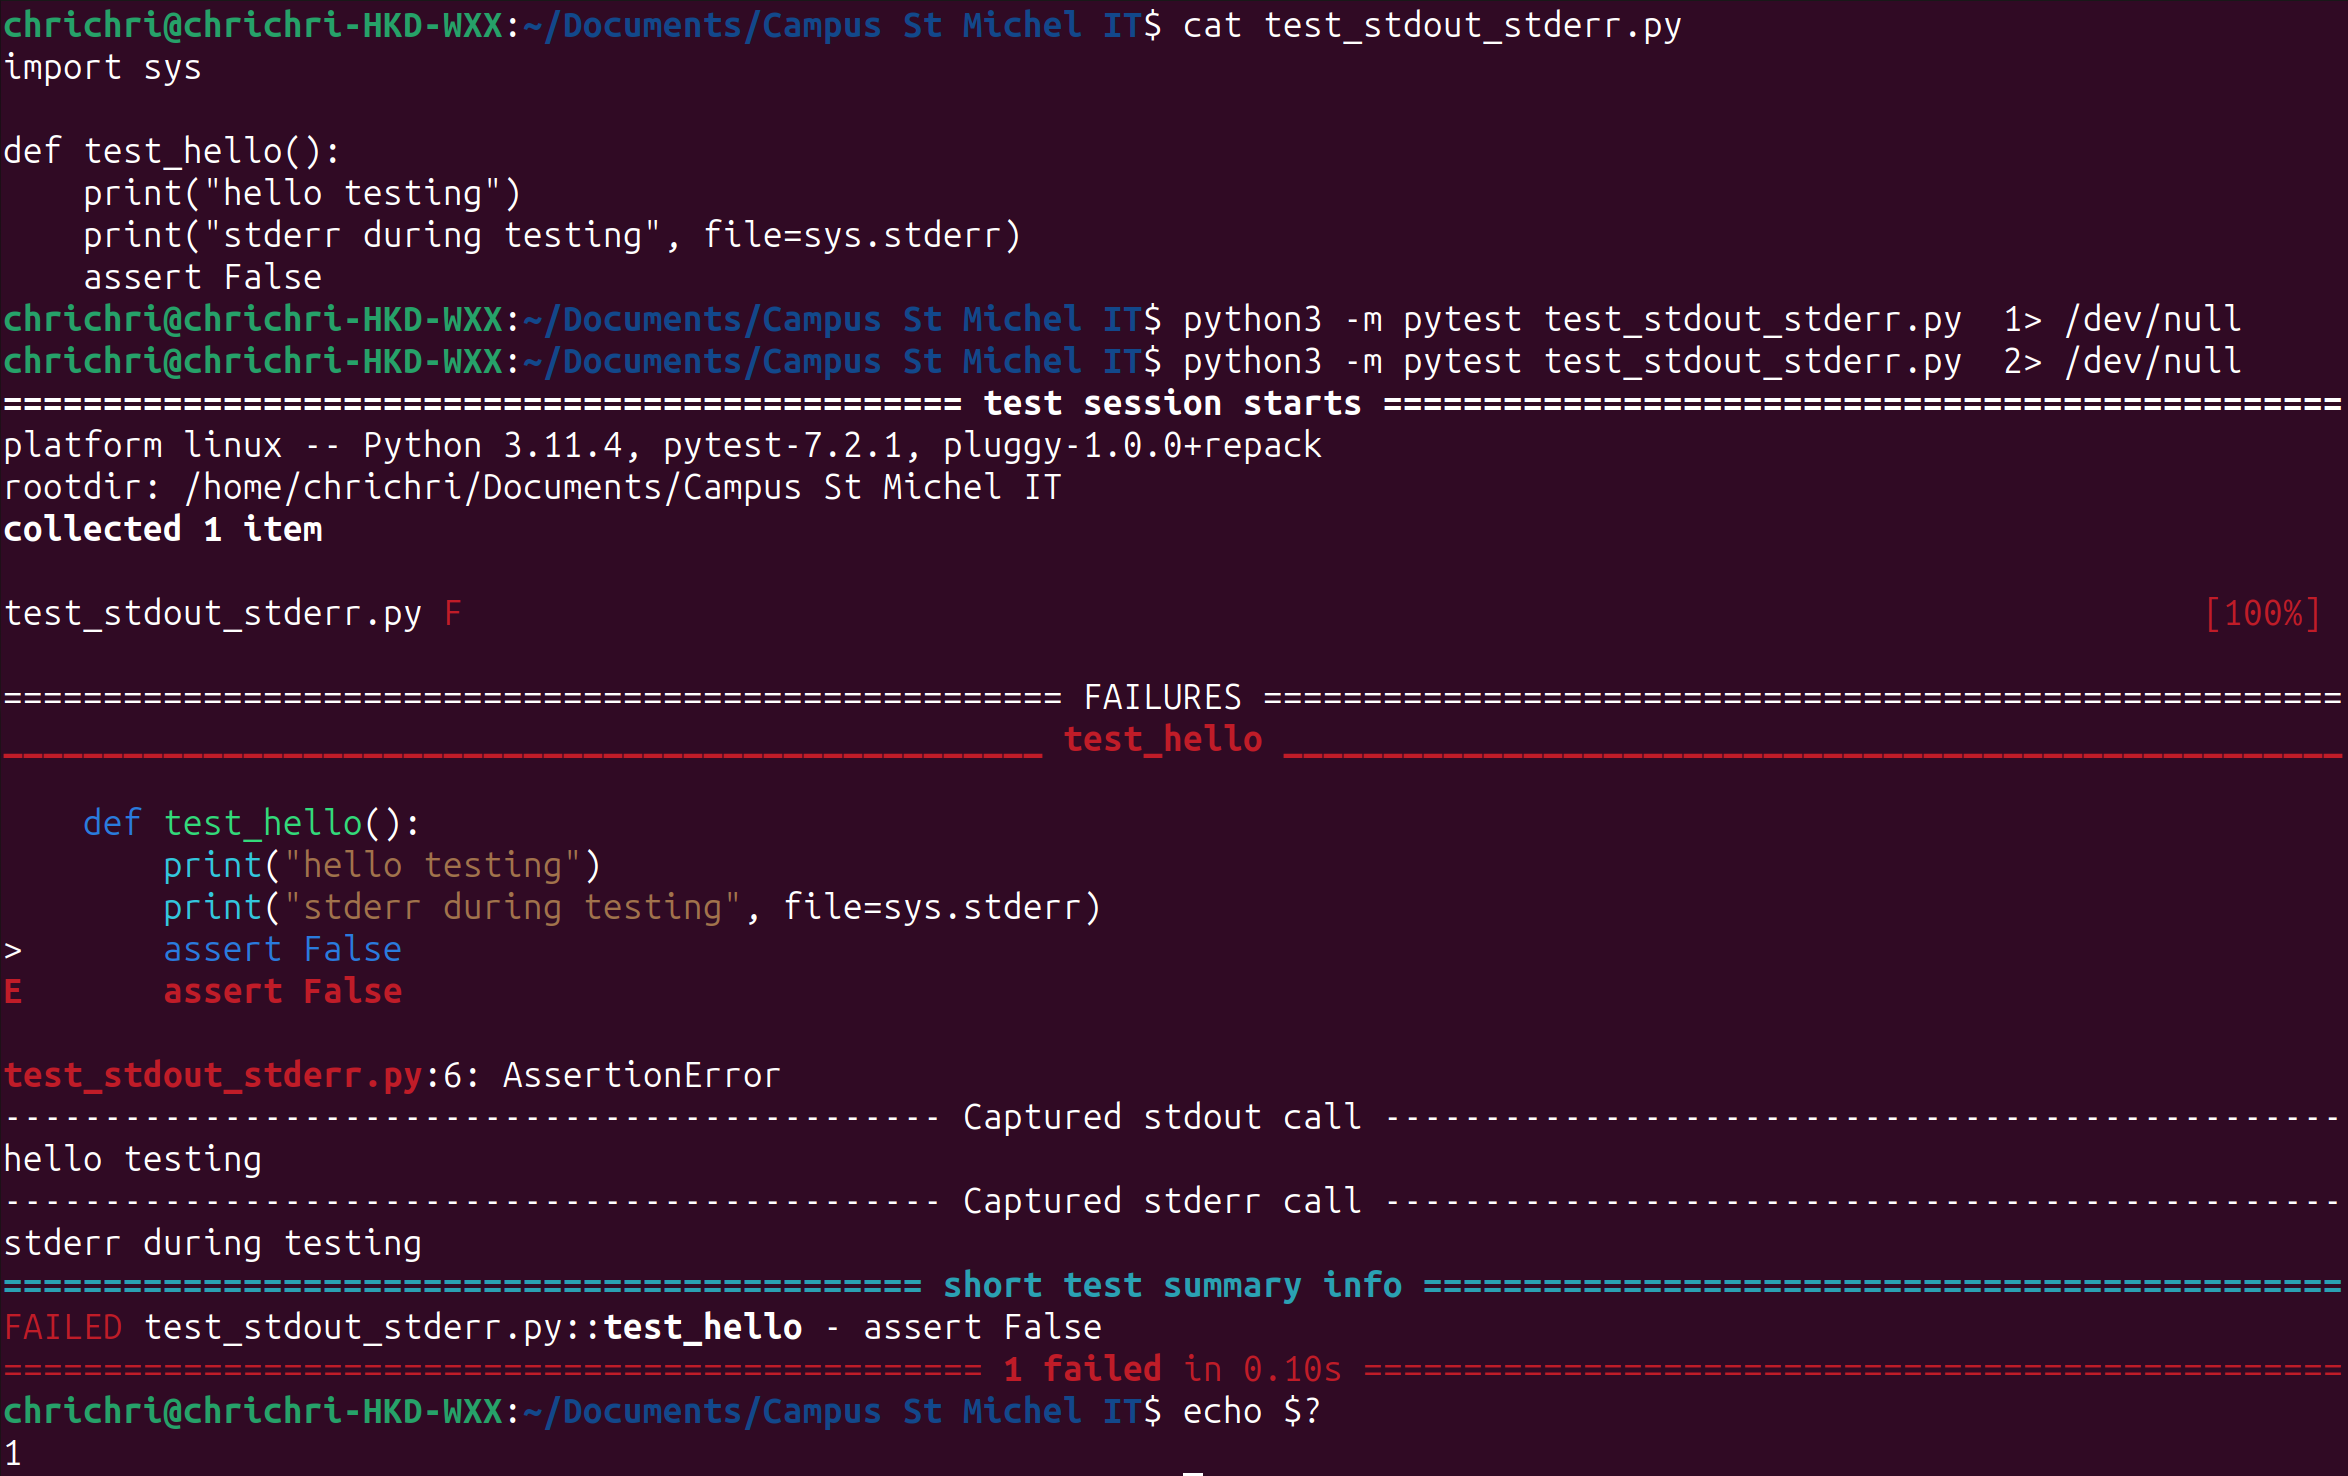
\includegraphics[width=7cm]{image/terminal-test-report}

    \end{frame}

    \begin{frame}{Brief sur les outils de test logiciel}
        \begin{itemize}
            \item Les frameworks de test retournent 3 statuts, OK, FAILED et ERROR~.

            \item OK si aucune erreur n’a lieu et FAILED en cas d’erreur d’assertion, \lstinline{AssertionError} en Python et Java.

            \item Pas de standard universellement accepté mais un format domine, le XML JUnit.
            Un XML le définit par la grammaire \url{https://windyroad.com.au/dl/Open\%20Source/JUnit.xsd}.

            \item Vient de l’écosystème Java avec le package du même nom, JUnit, mais est présent dans la plupart des frameworks de test comme PHPUnit, Pytest.

            \item L’interopérabilité entre les outils est permise par cette XSD commune, mais pas plus de contrainte.
            Par exemple, l’interopérabilité entre les frameworks de test et les outils de CI/CD~.

            \item Certains outils, souvent des solutions propriétaires, rechignent toujours à exporter un JUnit contenant les résultats de test pour fermer leur environnement.

        \end{itemize}
    \end{frame}


    \begin{frame}[fragile]{L'assertion error}{En Python}
        \transdissolve
        L’instruction \lstinline{assert} vérifie une condition.
        Si la condition est vraie, cela ne fait rien et votre programme continue simplement à s’exécuter.
        Mais si la condition d’assertion est fausse, elle lève une exception \lstinline{AssertionError}.
        \begin{lstlisting}[language=Python]
assert 23 % 2 == 0, "Le restant de la division est différent de 0"
        \end{lstlisting}
        Étant toujours fausse, le programme crash.
        \begin{lstlisting}[language=sh]
chrichri@chrichri-HKD-WXX:~$ python3 -c 'assert 23 % 2 == 0, "Le restant de la division est différent de 0"'
Traceback (most recent call last):
  File "<string>", line 1, in <module>
AssertionError: Le restant de la division est différent de 0
        \end{lstlisting}
    \end{frame}

    \begin{frame}{Pourquoi Pytest pour le testing}
        \transdissolve
        \textquote{pytest is a mature full-featured Python testing tool that helps you write better programs.\footnote{pytest: helps you write better programs , \url{https://docs.pytest.org}}}
        \begin{columns}
            \column{0.6\textwidth}
            Pytest est le framework de test en Python le plus utilisé selon les sondages de JetBrains\footnotemark.

            Seuls JUnit et Pytest sont pour tous usages, les autres sont orientés web.
            \column{0.4\textwidth}
            \centering
            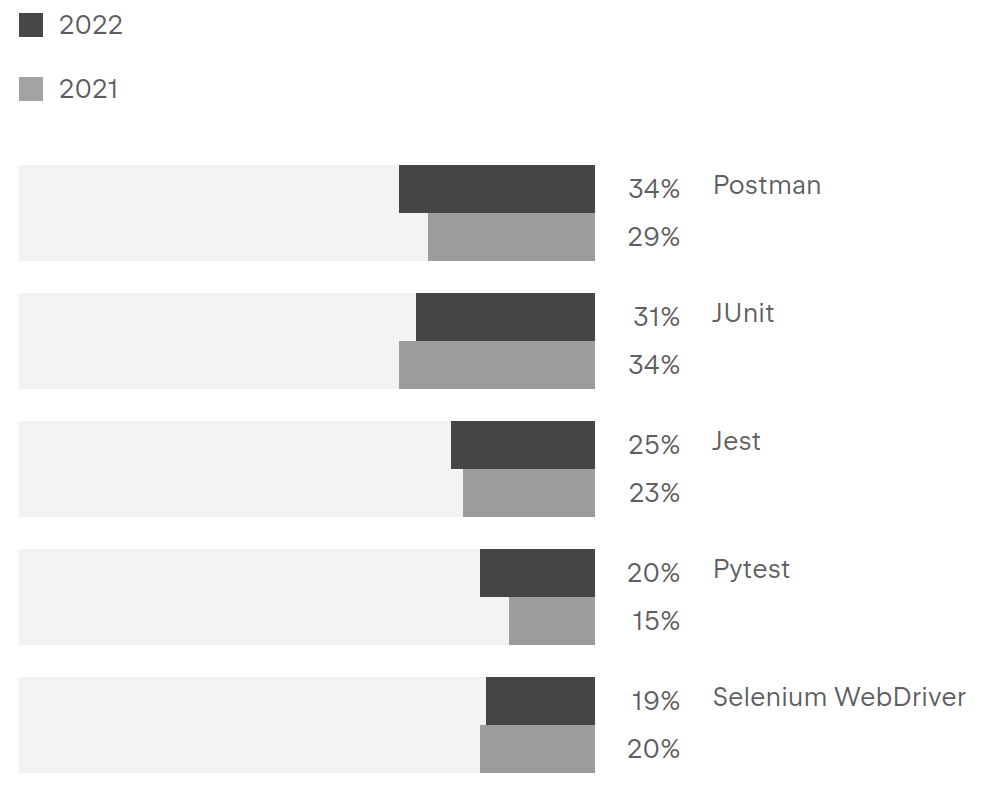
\includegraphics[width=5cm]{image/jetbrains-survey-testing-framework}
        \end{columns}
        \footnotetext{JetBrains, Which test frameworks , \url{https://www.jetbrains.com/lp/devecosystem-2022/testing/}}

    \end{frame}

    \begin{frame}[fragile]{Pytest}{Rédiger un test}
        \transdissolve
        \begin{itemize}
            \item Un module de test Pytest est un module Python préfixé par \lstinline{test_}.

            \item Toutes les méthodes préfixées par \lstinline{test_} sont exécutées par Pytest.
            Qu'elles soient dans une classe ou non.
            Les autres méthodes ne sont exécutées uniquement si les tests les appellent.
        \end{itemize}
        Ici par exemple, la précédente assertion est intégrée dans une méthode nommée \lstinline{test_divide} dans le module de test \lstinline{test_division.py}.
        \begin{lstlisting}[language=Python]
def test_divide():  # Un test Pytest est préfixé par test_
    assert 23 % 2 == 0, "Le restant de la division est différent de 0."
        \end{lstlisting}
    \end{frame}


    \begin{frame}[fragile]{Pytest}{Lancer les tests}
        \transdissolve
        Lancer avec la commande \lstinline{python -m pytest test_divison.py}, Pytest affiche le rapport de test.
        \begin{lstlisting}[language=sh]
...
def test_divide():  # Un test Pytest est préfixé par test_
>       assert 23 % 2 == 0, "Le restant de la division est différent de 0."
E       AssertionError: Le restant de la division est différent de 0.
E       assert (23 % 2) == 0

test_divison.py:2: AssertionError
...
        \end{lstlisting}

        De très utiles et nombreuses options peuvent compléter cette ligne de commande.
        Pour les découvrir, lancez \lstinline{python -m pytest --help} et \textquote{RTFM}.
    \end{frame}

    \begin{frame}[fragile]{Pytest}{Les tests paramétriques}
        \transdissolve
        Les tests paramétriques sont des tests qui prennent un ensemble de paramètres en entrées.

        Ils permettent de tester plusieurs cas avec un seul test.

        Le rapport génère un cas de test par paramètre.
        Il est donc plus détaillé et permet de trouver
        les tests en échec plus facilement que si l'\lstinline {assert} était dans une boucle, ce qui ne donne qu'un statut OK ou Fail dans le rapport.
        \begin{lstlisting}[language=Python]
import pytest
...
@pytest.mark.parametrize("dividend", range(100))  # Paramétrage du test
def test_divide_from_0_to_99(dividend):  # Doit avoir un argument présent dans le paramétrage
    assert dividend % 2 == 0, "Le restant de la division est différent de 0."
        \end{lstlisting}
    \end{frame}

    \begin{frame}[fragile]{Pytest}{Les tests paramétriques}
        \transdissolve
        Génère 100 cas de tests.
        Met en évidence les dividendes dont le restant de la division par 2 est différent de 0, ici 1 par exemple.
        \begin{lstlisting}[language=sh]
collecting ... collected 100 items

test_divison.py::test_divide_from_0_to_99[0] PASSED                      [  1%]
test_divison.py::test_divide_from_0_to_99[1] FAILED                      [  2%]
test_divison.py:7 (test_divide_from_0_to_99[1])
1~!= 0

Expected~:0
Actual  ~:1
<Click to see difference>

dividend = 1

    @pytest.mark.parametrize("dividend", range(100))  # Paramétrage du test
    def test_divide_from_0_to_99(dividend):  # Doit avoir un argument présent dans le paramétrage
>       assert dividend % 2 == 0, "Le restant de la division est différent de 0."
E       AssertionError: Le restant de la division est différent de 0.
E       assert (1 % 2) == 0
        \end{lstlisting}
    \end{frame}

    \begin{frame}[fragile]{Pytest}{Plantage dans un test, quel statut~?}
        \transdissolve
        Ce test crash avant l'assert.
        \begin{lstlisting}[language=Python]
def test_fail_or_error():  # Une erreur donne un fail ou error?
    dividende = 23 / 0
    assert dividende % 2 == 0, \
        "Le restant de la division est différent de 0."
        \end{lstlisting}
        Malgré l'absence d'\lstinline{assertionError}, le test est en échec et non en erreur.
        \begin{lstlisting}[language=sh]
test_divison.py::test_fail_or_error FAILED                               [100%]
test_divison.py:12 (test_fail_or_error)
def test_fail_or_error():  # Une erreur donne un fail ou error?
>       dividende = 23 / 0
E       ZeroDivisionError: division by zero

test_divison.py:14: ZeroDivisionError
        \end{lstlisting}

        \begin{dangercolorbox}
            Pour éviter les faux négatifs, un test doit tendre, tant que faire se peut, vers un \lstinline{assert}.
            Pour cela pensez à utiliser les fonctions \lstinline{parametrize} et \lstinline{fixture}.
        \end{dangercolorbox}
    \end{frame}

    \begin{frame}[fragile]{Pytest}{Les fixtures}
        \transdissolve
        Cf. \url{https://github.com/St-Michel-IT/testing/blob/main/test_customer_database.py}

        Un \lstinline{return} ou un \lstinline{yield} envoie l'objet au test dans l'état voulu.
        \begin{lstlisting}[language=Python]
@pytest.fixture
def customer_without_table():
    """...
    """
    customer = Customer()  # Avant le test, c'est le setup
    yield customer  # Un yield évite de sortir de la fonction
    customer.con.close()  # Après le test, le teardown
        \end{lstlisting}
        Le test n'a qu'une seule ligne, qu'un \lstinline{assert} l'échec ne
        pourrait venir que de là.
        \begin{lstlisting}[language=Python]
def test_instantiation(customer_without_table):
    """...
    """
    assert isinstance(customer_without_table.con, Connection)
        \end{lstlisting}
        En cas de plantage dans la fixture, i.e., avant ou après le test, la sanction
        serait erreur et non échec.

        Le rapport reflétera fidèlement le test et sera exempt de faux négatif.
    \end{frame}

    \begin{frame}[fragile]{Pytest}{Les fixtures, le moyen du pattern A.A.A\footnote{Arrange-Act-Assert: A Pattern for Writing Good Tests, \url{https://automationpanda.com/2020/07/07/arrange-act-assert-a-pattern-for-writing-good-tests/}}}
        \transdissolve
        Le pattern du A.A.A, Arrange, Act, Assert, est facile à implémenter avec les fixtures.
        Arrange et Act sont isolé dans la fixture, Assert seul est dans le test.

        \begin{lstlisting}[language=Python]
def customer_without_table():
    """...
    """
    customer = Customer()  # Arrange et Act dans le setup avant yiel ou return
    yield customer
    customer.con.close()  # Pas de nom en A, ils l'ont oublié?
        \end{lstlisting}
        Le test tend vers un \lstinline{assert} quasi seul.
        \begin{lstlisting}[language=Python]
def test_instantiation(customer_without_table):
    """...
    """
    assert isinstance(customer_without_table.con, Connection) # Assert
        \end{lstlisting}
        Le B.D.D. suit le pattern A.A.A sous un autre nom~: Given-When-Then.
        Le langage Gherkin utilise les étapes Given-When-Then pour spécifier les comportements dans les scénarios.
    \end{frame}

    \begin{frame}[fragile]{Pytest}{Le scope des fixtures}
        \transdissolve
        L'argument \lstinline{scope} du décorateur \lstinline{pytest.fixture} défini la durée de vie
        de la fixture.
        Il peut prendre 3 valeurs~:
        \begin{itemize}
            \item \lstinline{function}~: La valeur par défaut si on ne met rien.
            La fixture est exécutée à chaque fonction de test \lstinline{def test_...} qui l'appelle directement ou indirectement, donc les éventuels setup et teardown de cette dernière aussi.
            \item \lstinline{module}~: Une fois par module \lstinline{test_....py}.
            \item \lstinline{session}~: Une seule fois durant la session de test quel que soit le nombre de modules et de tests exécutés.
        \end{itemize}
        \begin{lstlisting}[language=Python]
@pytest.fixture(scope="function")  # Scope de la fixture, par default function
def customer_without_table():
    """
    Connection to in memory database using the Customer class
        \end{lstlisting}

        Pour tester une API en étant sûr le token n'est pas périmé, on peut utiliser le scope \lstinline{function} pour en avoir un nouveau à chaque appel.

        Si préparer les conditions initiales, le setup, prend du temps, on évitera si possible de le répéter à chaque test avec les scopes \lstinline{module}, \lstinline{session}.
    \end{frame}

    \begin{frame}{Pytest}{\lstinline{Le conftest.py}}
        \transdissolve
        Il n'a qu'une seule particularité, c'est d'être importé automatiquement par Pytest lorsqu'il est présent dans le dossier courant des tests.

        Il permet de factoriser les fixtures et les paramétrages de tests utilisés dans plusieurs modules de tests, car ces derniers seront automatiquement disponibles sans même un import dans le module.
        \begin{columns}
            \column{0.5\textwidth}
            \dirtree{%
                .1 ./.
                .2 {conftest.py}.
                .2 {\textcolor{flatgreen}{test\_no\_directory.py}}.
                .2 unit.
                .3 {\textcolor{flatgreen}{test\_integration.py}}.
                .2 functional.
                .3 {\textcolor{flatgreen}{test\_functional.py}}.
            }\column
            {0.5\textwidth}
            Pour tous ces tests, s'ils sont lancés depuis la racine avec la commande \lstinline{pytest}, le \lstinline{conftest.py} sera importé automatiquement.
        \end{columns}
        \bigbreak
        \begin{columns}
            \column{0.9\textwidth}
            PyCharm intègre par défaut Pytest comme lanceur de tests et fournit l'autocomplétion pour les fixtures du \lstinline{conftest.py}.
            \column{0.1\textwidth}
            \centering
            
\includegraphics[width=1cm]{image/logo-pycharm}
        \end{columns}
    \end{frame}

    \begin{frame}[fragile]{Pytest}{Le coverage}
        \transdissolve
        Pas de support natif du coverage par Pytest, il faut installer le plugin \lstinline{pytest-cov}\footnote{Welcome to pytest-cov’s documentation!, \url{https://pytest-cov.readthedocs.io/en/latest/}}.

        Pour appeler le plugin, il faut passer en argument le module à tester et le(s) test(s) de ce dernier.


        \begin{lstlisting}[language=sh]
pytest --cov=\textcolor{flatgreen}{customer_database} ./test_customer_database.py
...
rootdir: /home/chrichri/Documents/Campus-St-Michel-IT/testing
plugins: cov-4.1.0
collected 6 items

test_customer_database.py ......                                                                                                                                                                                                 [100%]

---------- coverage: platform linux, python 3.11.4-final-0 -----------
Name                   Stmts   Miss  Cover
------------------------------------------
customer_database.py       9      0   100%
------------------------------------------
TOTAL                      9      0   100%
        \end{lstlisting}

    \end{frame}

    \begin{frame}{Pytest}{Le coverage}
        \transdissolve
        \begin{columns}

            \column{0.5\textwidth}
            \centering
            \includegraphics[width=5cm]{image/html-coverage}
            \column{0.5\textwidth}
            L'option \lstinline{--cov-report=html} permet de générer un rapport HTML plus détaillé qui met en lumière quelles parties du code sont couvertes par les tests et lesquelles ne le sont pas.
            \bigbreak
            \textbf{Exercice}~: Trouvez quel test du module \url{https://github.com/St-Michel-IT/testing/blob/main/test_customer_database.py} couvre quelle partie de ce code~:
        \end{columns}

    \end{frame}

    \begin{frame}{Pytest}{Le secret de la réussite}
        \transdissolve
        \begin{columns}
            \column{0.7\textwidth}
            Pytest est un framework complet voir complexe.

            Mais quasi toutes les fonctionnalités auxquelles on peut penser sont déjà implémentées et décrites une documentation de qualité.

            Comme avec toutes les grosses libraries, il faut avoir confiance en leur design et chercher dedans avant de réinventer la roue.

            La liste des fonctionnalités est trop longue, nous venons juste d'en découvrir les principales.
            \bigbreak
            Donc une fois encore, comme pour toutes les bonnes libraires à connaître, le secret est \textquote{\textbf{\Large{RTFM}}}~!
            \column{0.3\textwidth}
            \centering
            \includegraphics[width=3cm]{image/girl-rtfm}
        \end{columns}
    \end{frame}


    \section{Versionning (GIT)}\label{sec:versionning-(git)}

    \begin{frame}{Qu'est-ce que Git~?}
        \transdissolve
        Caractéristiques principales de Git~:
        \begin{itemize}
            \item C'est un protocole de gestion de versions décentralisé, A.K.A. Distributed Version Control System (DVCS).
            Décentralisé car chaque utilisateur a une copie complète du dépôt et de l'historique.
            \item Protocole au dessus de HTTP ou de SSH. Le plus souvent utilisé avec SSH, car plus sécurisé.
            \item Utilisé par les serveurs GitHub, GitLab, Bitbucket, Gitee, etc.
            Ne pas confondre Git et GitHub, ce sont deux choses distinctes, l'un est le protocole, l'autre sont implémentation dans un serveur à des fins commerciales.
            \item Il est open source et donc gratuit.
            \item L'intégrité de tout objet est vérifiée par SHA-1
            \item \textquote{Git is easy to learn}\footnote{git, \url{https://git-scm.com/}} \emoji{smiling-face-with-halo}
        \end{itemize}
    \end{frame}

    \begin{frame}{Qu'est-ce que Git~?}{L'histoire de Git\footnote{A Short History of Git, \url{https://git-scm.com/book/en/v2/Getting-Started-A-Short-History-of-Git}}}
        \transdissolve
        Linus Torvalds, le créateur de Linux, a créé Git en 2005 pour gérer le code source du noyau Linux.
        BitKeeper, un VCS propriétaire, était utilisé avant, mais la licence gratuite a été révoquée par l'éditeur.
        \smallbreak
        \begin{columns}
            \column{0.6\textwidth}
            Torvalds souhaite développer un VCS libre et gratuit, avec les qualités suivantes~:
            \begin{itemize}
                \item Speed
                \item Simple design
                \item Strong support for non-linear development (thousands of parallel branches)
                \item Fully distributed
                \item Able to handle large projects like the Linux kernel efficiently (speed and data size)
            \end{itemize}
            \column{0.4\textwidth}
            \centering
            \includegraphics[width=4.5cm]{image/linus-quote.jpeg}
        \end{columns}
    \end{frame}

    \begin{frame}{Qu'est-ce que Git~?}{Extraits du manuel Git\cref{progit}]}
        \transdissolve
        Le code source n'est qu'en un seul exemplaire sur le file system mais une base de données complète est présente sur chaque poste de travail.
        Elle est dans le \lstinline{.git} à la racine du projet.
        \bigbreak
        \centering
        \includegraphics[width=6cm]{image/git-local-history}
    \end{frame}

    \begin{frame}{Qu'est-ce que Git~?}{Extraits du manuel Git\cref{progit}}
        \transdissolve
        Le \textquote{checkout} est l'action de déployer en local une branche de code.

        Le \textquote{staging} est l'action de désigner un fichier modifié comme faisant partie de la prochaine version, i.e., du prochain \textquote{commit}.
        \bigbreak
        \centering
        \includegraphics[width=8cm]{image/git-local-areas}
    \end{frame}

    \begin{frame}{Qu'est-ce que Git~?}{Extraits du manuel Git\footnote{\label{progit}Pro Git, \url{https://git-scm.com/book/en/v2}}}
        \transdissolve
        Les développeurs peuvent travailler sur les mêmes fichiers en parallèle.
        Chaque développeur peut même recréer un serveur en cas de disparition du serveur.
        \bigbreak
        \centering
        \includegraphics[width=5cm]{image/dvcs-scheme}
    \end{frame}

    \begin{frame}{Les interfaces de Git}{\lstinline{gitk}, le GUI\footnote{Git in Other Environments - Graphical Interfaces, \url{https://git-scm.com/book/en/v2/Appendix-A:-Git-in-Other-Environments-Graphical-Interfaces}}}
        \transdissolve
        C'est principalement un navigateur de l'historique des commits du repository.
        Il se lance avec la commande \lstinline{gitk}.
        \bigbreak
        \centering
        \includegraphics[width=6cm]{image/gitk}
    \end{frame}

    \begin{frame}{Les interfaces de Git}{\lstinline{git}, la CLI\footnote{Embedding Git in your Applications - Command-line Git, \url{https://git-scm.com/book/en/v2/Appendix-B:-Embedding-Git-in-your-Applications-Command-line-Git}}}
        \transdissolve
        C'est l'implémentation la plus orthodoxe.
        Elle porte absolument toutes les fonctionnalités, ce qui n'est pas le cas des autres.
        \bigbreak
        \centering
        \includegraphics[width=5cm]{image/git-cli-help}
    \end{frame}

    \begin{frame}{Les interfaces de Git}{Git dans votre IDE préféré}
        \transdissolve
        Disponible dans les IDEs Jetbrains, VS Code et probablement la plupart des IDEs modernes.
        Par exemple, au plus près du code Python dans PyCharm~:
        \bigbreak
        \centering
        \includegraphics[width=10cm]{image/git-in-pycharm}
    \end{frame}

    \begin{frame}{Les interfaces de Git}{Les API git dans la pluspart des langages de programmation}
        \transdissolve
        Pour intégrer la version dans des rapports de tests, dans un souci de traçabilité par exemple.
        Le script de test peut appeler l'API pour avoir le hash du commit en cours de test.

        Il peut même être afficher dans soft dans un souci de transparence, c'est le hash versioning.
        \bigbreak
        \begin{columns}
            \column{0.5\textwidth}
            Exemple de libraires~:
            \begin{itemize}
                \item Libgit2 pour le C/C++
                \item JGit pour le Java
                \item go-git, pour le Go
                \item Dulwich pour Python
            \end{itemize}
            \column{0.5\textwidth}
            \centering
            \includegraphics[width=5cm]{image/code-scrutiny}
        \end{columns}
    \end{frame}

    \begin{frame}[fragile]{Git, les actions et leurs commandes}{Etape 1, récupérer les sources et l'historique d'un repository existant\footnote{\label{progitgetrepo}Git Basics - Getting a Git Repository, \url{https://git-scm.com/book/en/v2/Git-Basics-Getting-a-Git-Repository}}}
        \transdissolve
        Pour récupérer le code d'un sur Github par exemple, il suffit de cliquer sur le bouton \textquote{Code} et de copier l'URL du protocole HTTPS ou SSH si authentifié avec des clés SSH~.

        La commande suivante va cloner le repository dans le dossier courant en ajoutant le \lstinline{.git} et les sources~:
        \begin{lstlisting}[language=sh]
$ git clone <URL>
        \end{lstlisting}
        \begin{columns}
            \column{0.5\textwidth}
            Par exemple les ~7 Go du noyau Linux~!
            \column{0.5\textwidth}
            \centering
            \includegraphics[width=3cm]{image/git-clone-artwork}
        \end{columns}
    \end{frame}

    \begin{frame}[fragile]{Git, les actions et leurs commandes}{Etape 1, si le repo n'existe pas, qu'on le créé\cref{progitgetrepo}\footnote{Git remote, \url{https://git-scm.com/docs/git-remote}}}
        \transdissolve
        Si le repo n'existe pas, que le projet démarre de zéro, il faut initialiser le dépôt avec les commandes suivantes~:
        \begin{lstlisting}[language=sh]
$ mkdir mon-nouveau-projet
$ cd mon-nouveau-projet
$ git init
$ git add *.c
$ git add LICENSE
$ git commit -m 'Initial project version'
        \end{lstlisting}

        Pour ajouter un dépôt distant (sur le un serveur comme Github par exemple), on peut utiliser la commande~:
        \begin{lstlisting}[language=sh]
$ git remote add -f -t master -m master origin <URL>
        \end{lstlisting}
    \end{frame}

    \begin{frame}[fragile]{Git, les actions et leurs commandes}{Le local et le remote sont bien différents\footnote{\label{progitfetch}Fetching changes from a remote repository, \url{https://docs.github.com/en/get-started/using-git/getting-changes-from-a-remote-repository\#fetching-changes-from-a-remote-repository}}}
        \transdissolve
        Le dépôt local est donc lié à un server distant (GitHub, Gitlab, Bitbucket, etc), le \textquote{remote}.
        Il faut bien comprendre que ces deux pools de code peuvent être dans des états bien différents.

        Sans action sur le local, les changements (évolution du code, création de branche, etc) du \textquote{remote} ne sont pas connus en local.
        Il faut donc les récupérer avec la commande suivante~:
        \begin{lstlisting}[language=sh]
$ git fetch
        \end{lstlisting}
        La commande \lstinline{fetch} ne \textquote{merge} pas, i.e., ne fusionne pas les modifications du serveur distant.

        Plus de détails dans Git Pro book\footnote{Git Basics - Recording Changes to the Repository, \url{https://git-scm.com/book/en/v2/Git-Basics-Recording-Changes-to-the-Repository}}.

    \end{frame}


    \begin{frame}[fragile]{Git, les actions et leurs commandes}{Créer une version à partir des changements locaux\cref{progitfetch}}
        \transdissolve

        Pour ajouter un nouveau fichier source ou \textquote{stage} un fichier modifié, on peut utiliser la commande~:
        \begin{lstlisting}[language=sh]
$ git add <fichier source>
        \end{lstlisting}

        Les modifications qui ne sont pas stage ne feront pas partie de la prochaine version et ne pourront donc être poussées sur le serveur


        Pour créer une version à partir des changements locaux avec un message, on peut utiliser la commande~:

        \begin{lstlisting}[language=sh]
$ git commit -m "<Message de commit>"
        \end{lstlisting}

        Il est aussi possible de stage automatiquement toutes les modifications lors du \lstinline{commit} avec l'option \lstinline{-a} comme all, pour gagner du temps.

        \begin{lstlisting}[language=sh]
$ git commit -a -m "<Message de commit>"
        \end{lstlisting}
    \end{frame}



    \begin{frame}[fragile]{Git, les actions et leurs commandes}{Créer une version à partir des changements locaux\cref{progitfetch}}
        \transdissolve

        Avant un commit, pour suivre les modifications, lesquelles sont \textquote{stage} et lesquelles ne le sont pas, on peut utiliser la commande~:
        \begin{lstlisting}[language=sh]
$ git status
Sur la branche master
Votre branche est à jour avec 'origin/master'.

Modifications qui seront validées :
  (utilisez "git restore --staged <fichier>..." pour désindexer)
        modifié :         "doc/Qualit\303\251-Code-Source-L3-CSI.tex"

Modifications qui ne seront pas validées :
  (utilisez "git add <fichier>..." pour mettre à jour ce qui sera validé)
  (utilisez "git restore <fichier>..." pour annuler les modifications dans le répertoire de travail)
        modifié :         "doc/build/pdf/Qualit\303\251-Code-Source-L3-CSI.pdf"

Fichiers non suivis:
  (utilisez "git add <fichier>..." pour inclure dans ce qui sera validé)
        .idea/
        \end{lstlisting}

    \end{frame}

    \begin{frame}{Git, les actions et leurs commandes}{Créer une version à partir des changements locaux\cref{progitfetch}}
        \transdissolve

        Les différents status d'une source sont donc~:

        \begin{center}
            \includegraphics[width=10cm]{image/git-lifecycle}
        \end{center}

        \begin{dangercolorbox}
            Les bonnes pratiques veulent qu'on ne suit pas, i.e., on ne \textquote{stage} pas les fichiers de configuration pour des raisons de sécurité, de données hors jeux de test, de fichier généré (build, log, cache, fichier temporaire, documentation générée, etc).
        \end{dangercolorbox}
    \end{frame}


    \begin{frame}[fragile]{Git, les actions et leurs commandes}{Créer une version à partir des changements locaux\footnote{Git Basics - Viewing the Commit History, \url{https://git-scm.com/book/en/v2/Git-Basics-Viewing-the-Commit-History}}}
        \transdissolve

        La version est identifiée par un hash, le \textquote{commit hash}.
        Calculé par la fonction de hashage SHA-1, il est unique pour chaque version.

        Des commandes permettent de lire l'historique des versions locales, comme par exemple~:
        \begin{lstlisting}[language=sh]
$ git log
commit 43c417023f1b6277a996cb32843bd6fe955e5aea (HEAD -> master, origin/master)
Author: chrichri <christophe.brun@papit.fr>
Date:   Sun Feb 11 01:19:44 2024 +0100

    PDF re-built.

commit 5d939ba92563d9110e5dcf3207d87e383743b33c
Author: chrichri <christophe.brun@papit.fr>
Date:   Sun Feb 11 01:18:16 2024 +0100

    Add missing images.
        \end{lstlisting}
    \end{frame}


    \begin{frame}[fragile]{Git, les actions et leurs commandes}{Pousser la version locale sur le serveur\footnote{\label{progitpushing}Git Basics - Working with Remotes, \url{https://git-scm.com/book/en/v2/Git-Basics-Working-with-Remotes\#_pushing_remotes}}}
        \transdissolve


        \begin{columns}
            \column{0.7\textwidth}
            Pour pousser la version locale sur le serveur, sur la même branche que la locale, on peut utiliser la commande~:
            \begin{lstlisting}[language=sh]
$ git push
            \end{lstlisting}
            \column{0.3\textwidth}
            \centering
            \begin{center}
                \includegraphics[width=3cm]{image/schematic-drawing-of-a-computer-linked-to-a-remote-server}
            \end{center}
        \end{columns}

        Pour pousser une branche locale spécifique, on peut utiliser la commande~:
        \begin{lstlisting}[language=sh]
$ git push origin <nom-de-branche>
        \end{lstlisting}
        Pour pousser une branche locale sur une branche distante différente, on peut utiliser la commande~:
        \begin{lstlisting}[language=sh]
$ git push origin <nom-de-branche-locale>:<nom-de-branche-distante>
        \end{lstlisting}

        Un merge donne lieu à une fusion en mode \textquote{fast-forward}.
    \end{frame}

    \begin{frame}[fragile]{Git, les actions et leurs commandes}{Tirer les modifications du serveur sur le dépôt local\cref{progitpushing}\footnote{Merge, Fast-Forward et rebase: un peu de culture git,\url{https://www.dynamic-mess.com/developpement/git-merge-fast-forward-rebase-culture-git/}}}
        \transdissolve

        Pour tirer du code distant dans le dépôt local, une commande possible est~:
        \begin{lstlisting}[language=sh]
$ git pull
        \end{lstlisting}

        Suite à cette commande, il y a trois cas de figure~:
        \begin{itemize}
            \item S'il y a des différences entre les codes, elles sont mergés avec ou sans \textquote{fast-forward}.
            Le \textquote{fast-forward} est juste une façon de construire l'historique des modifications sans commit de merge.
            Par défaut il y a \textquote{fast-forward}, pour avoir le commit de merge il faut ajouter l'option \lstinline{--no-ff}.
            \item Si le dépôt local n'a pas été modifié depuis le dernier \lstinline{fetch}, le \lstinline{pull} est un simple \lstinline{fast-forward}.
            \item S'il y a conflict, c'est à dire que des mêmes lignes ont été modifiés en parallèle, il faut les résoudre avant de pouvoir \lstinline{commit}\footnote{Conflits de merge Git, url{https://www.atlassian.com/fr/git/tutorials/using-branches/merge-conflicts}}.
        \end{itemize}
    \end{frame}

    \begin{frame}{Git, les actions et leurs commandes}{Tirer les modifications du serveur sur le dépôt local\footnote{Merge, Fast-Forward et rebase: un peu de culture git,\url{https://www.dynamic-mess.com/developpement/git-merge-fast-forward-rebase-culture-git/}}}
        \transdissolve

        Différence, \lstinline{fast-forward} et commit de merge, seul l'historique change pas le code~:
        \begin{center}
            \includegraphics[width=10cm]{image/fast-forward-merge}
        \end{center}
    \end{frame}


    \begin{frame}[fragile]{Git, les actions et leurs commandes}{Tirer les modifications du serveur sur le dépôt local\footnote{Merge, Fast-Forward et rebase: un peu de culture git,\url{https://www.dynamic-mess.com/developpement/git-merge-fast-forward-rebase-culture-git/}}}
        \transdissolve

        Pour tirer du code distant dans le dépôt local, une commande est possible est~:
        \begin{lstlisting}[language=sh]
$ git rebase
        \end{lstlisting}

        Le \lstinline{rebase} est une autre façon de construire l'historique des modifications sans commit de merge.
        Les modifications sont placées à la fin de l'historique, ce qui donne un historique plus lisible.
        \begin{columns}
            \column{0.5\textwidth}
            \begin{center}
                \includegraphics[width=5cm]{image/git-rebase}
            \end{center}
            \column{0.5\textwidth}
            Tout comme avec le \lstinline{pull}, il peut y avoir des conflits à résoudre.
            Une fois cela resolu il faut \lstinline{commit} les modifications.
            Puis terminer le \lstinline{rebase} avec la commande avec \lstinline{git rebase --continue}\footnotemark.
        \end{columns}
        \footnotetext{Resolving merge conflicts after a Git rebase, \url{https://docs.github.com/en/get-started/using-git/resolving-merge-conflicts-after-a-git-rebase}}
    \end{frame}

    \begin{frame}[fragile]{Git, les actions et leurs commandes}{Le branching\footnote{\label{progitmerge}Git Branching - Basic Branching and Merging,\url{https://git-scm.com/book/en/v2/Git-Branching-Basic-Branching-and-Merging}}}
        \transdissolve

        Pour passer d'une branche à l'autre dans le dépôt local, la commande est~:
        \begin{lstlisting}[language=sh]
$ git checkout <nom-de-branche>
        \end{lstlisting}

        Pour créer une nouvelle branche à partir de la branche courante et passer dessus, rajouter l'option \lstinline{-b}~:
        \begin{lstlisting}[language=sh]
$ git checkout -b <nom-de-branche-à-créer>
        \end{lstlisting}

        Pour supprimer une branche, rajouter l'option\lstinline{-d}~:
        \begin{lstlisting}[language=sh]
$ git branch -d <nom-de-branche-à-supprimer>
        \end{lstlisting}

        Pour fusionner une autre branche locale dans la branche courante, la commande est~:
        \begin{lstlisting}[language=sh]
$ git merge <nom-de-branche-àmerger>
        \end{lstlisting}
    \end{frame}

    \begin{frame}[fragile]{Git, les actions et leurs commandes}{Le branching\cref{progitmerge}}
        \transdissolve

        La fusion de code, appelée \textquote{merge}, peut être effectuée automatiquement par \lstinline{git}.
        \begin{lstlisting}[language=sh]
$ git checkout master
$ git merge hotfix
Updating f42c576..3a0874c
Fast-forward
        \end{lstlisting}

        Des lignes modifiées dans les deux branches sont en conflit, \lstinline{git} donne les instructions de résolution~:
        \begin{lstlisting}[language=sh]
$ git merge iss53
Auto-merging index.html
CONFLICT (content): Merge conflict in index.html
Automatic merge failed; fix conflicts and then commit the result.
$ git status
On branch master
All conflicts fixed but you are still merging.
  (use "git commit" to conclude merge)
Changes to be committed:
    modified:   index.html
        \end{lstlisting}
    \end{frame}

    \begin{frame}[fragile]{Git, les actions et leurs commandes}{Le branching\cref{progitmerge}}
        \transdissolve

        En cas de \textquote{conflict}, \lstinline{git} ajoute des marqueurs de résolution de conflict.
        Ils permettent de voir les différences entre les deux branches et de choisir la version à conserver ou de créer un mélange des deux.
        \begin{lstlisting}[language=sh]
<<<<<<< HEAD:index.html
<div id="footer">contact : email.support@github.com</div>
=======
<div id="footer">
 please contact us at support@github.com
</div>
>>>>>>> iss53:index.html
        \end{lstlisting}
        A noter, qu'évidement, ils cassent toutes les syntaxes de tous les langages de programmation.
        On ne peut donc pas les oublier.
    \end{frame}

    \begin{frame}{Git, les actions et leurs commandes}{Pourquoi créer une branche~?}
        \transdissolve
        \begin{columns}
            \column{0.5\textwidth}
            \begin{center}
                \includegraphics[width=5cm]{image/schematic-drawing-of-git-branches}
            \end{center}
            \column{0.5\textwidth}
            \begin{itemize}
                \item Pour développer une nouvelle fonctionnalité sans perturber le code en production.
                \item Pour développer une correction de bug sans perturber le code en production.
            \end{itemize}
        \end{columns}
        Les bonnes pratiques sont qu'une branche a un nom qui explicite le but du développement.

        Son périmètre est restreint pour éviter les conflits de fusion et les codes review trop complexes lors de la pull request.
    \end{frame}

    \begin{frame}[fragile]{Git, les actions et leurs commandes}{Patchning avec \lstinline{git rebase}\footnote{\label{progitpatching}Git Commands - Patching, \url{https://git-scm.com/book/en/v2/Appendix-C:-Git-Commands-Patching}}}
        \transdissolve
        Avec \lstinline{git rebase}, on peut patcher n'importe quel commit et modifier l'historique des commits.

        Par exemple pour les 5 derniers commits~:
        \begin{lstlisting}[language=sh]
$ git rebase -i HEAD~5
pick 6a1c95c A bit more Git slides.
pick 5d939ba Add missing images.
pick 43c4170 PDF re-built.
pick 88d6af7 More Git.
pick f820b3e Almost the end of Git

# Rebasage de 49cc10e..f820b3e sur 49cc10e (5 commandes)
#
# Commands:
# p, pick <commit> = use commit
# r, reword <commit> = use commit, but edit the commit message
# e, edit <commit> = use commit, but stop for amending
# s, squash <commit> = use commit, but meld into previous commit
...
        \end{lstlisting}
    \end{frame}

    \begin{frame}{Git, les actions et leurs commandes}{Patchning avec \lstinline{git rebase}\cref{progitpatching}}
        \transdissolve
        \begin{itemize}
            \item \textquote{pick} pour garder le commit tel quel.
            \item \textquote{reword} pour modifier le message du commit, si le message n'est pas explicite.
            \item \textquote{edit} pour modifier le code du commit, en cas de bug par exemple.
            \item \textquote{squash} pour fusionner le commit avec le précédent.
            Souvent utilisé pour amener de la clarté dans l'historique en diminuant le nombre de message.
            \item \textquote{drop} Si une modification, i.e., un commit, n'a plus lieu d'être.
        \end{itemize}
    \end{frame}

    \begin{frame}{Git, le workflow}{Les pull requests, A.K.A PR\footnote{GitHub - Contributing to a Project\url{https://git-scm.com/book/en/v2/GitHub-Contributing-to-a-Project}}}
        \transdissolve
        Deux pools de code venant de branche ou d'un fork différent du même dépôt peuvent être fusionnées \textquote{merge} sur le serveur.
        \bigbreak
        Si on est contributeur dans le même dépôt, c'est une pull request d'une branche dans une autre.
        Sinon, si on est pas contributeur on peut proposer une pull request d'un fork dans le dépôt original.
        \bigbreak
        Une page synthétise les différences et permet de discuter des modifications, avant de valider ou non la PR~.
        \bigbreak
        En cas de souci lors de la revue, les autres développeurs expliquent les modifications à apporter pour que la PR soit acceptée et la refuse. \emoji{cross-mark}

        Une fois la PR revue et validée par une cohorte minimale de développeurs, le code est fusionné dans la branche cible. \emoji{check-mark}
    \end{frame}

    \begin{frame}{Git, le workflow}{Les pull requests, schéma récapitulatif\footnote{GitHub Pull request flow. \url{https://www.researchgate.net/figure/GitHub-Pull-request-flow_fig1_326295010}}}
        \transdissolve
        \begin{center}
            \includegraphics[width=10cm]{image/github-pull-request-flow}
        \end{center}
    \end{frame}

    \begin{frame}{Git, travaux dirigés}{Utilisé le \lstinline{clone}, le \lstinline{branch}, le \lstinline{push} et faire une PR}
        \transdissolve
        Chaque étudiant d'un groupe doit tirer le code du dépôt, écrire un nouveau test dans sa branche, le pousser sur le serveur et faire une PR~.
        \bigbreak
        La PR se fait de la branche de l'étudiant vers la branche \textquote{main} du dépôt.
        \bigbreak
        C'est le critère d'évaluation de la compréhension de la gestion de version avec Git.
    \end{frame}


    \section{Plateforme d’intégration et de livraisons continues}\label{sec:plateforme-dintegration-et-de-livraisons-continues}

    \begin{frame}{Intégration et livraisons continues A.K.A. CI/CD}{Les defintions du CI/CD}
        \transdissolve
        CI/CD est l'acronyme de \textquote{Continuous Integration/Continuous Delivery} ou \textquote{Continuous Deployment}.
        \bigbreak
        \textquote{le but ultime du processus CI/CD qui consiste à supprimer l’intervention humaine pour gagner en temps et en efficacité. Le code est compilé et testé sur l’ordinateur grâce à ce que l’on appelle un build automatisé. S’il n’y a pas de bug le tout est mis en production automatiquement. Cette approche permet aux développeurs de se concentrer sur la conception et le développement et sur les fonctionnalités de l’application.}\footnote{Qu'est-ce que l'approche CI/CD - Qu’est-ce que le processus CI/CD ?, \url{https://www.oracle.com/fr/cloud/definition-approche-ci-cd/}}
        \bigbreak
        \centering
        \includegraphics[width=7cm]{image/ci-cd-flow}
    \end{frame}

    \begin{frame}{Intégration et livraisons continues A.K.A. CI/CD}{Les defintions du CI/CD}
        \transdissolve
        Plusieurs remarques~:
        \begin{itemize}
            \item Une des avancées est l'automatisation de multiples tâches.
            \item Le mot intégration fait penser qu'on a plusieurs systèmes, logiciels, développeurs, équipes, etc.
            \item L'\textquote{ordinateur} n'est pas défini, on verra qu'il peut être celui du développeur ou un serveur distant voir un ordinateur inconnu.
            \item \textquote{S’il n’y a pas de bug le tout est mis en production automatiquement.} vous y croyez~?
            \item Le but est toujours le même, éliminer un maximum de bug.
        \end{itemize}
        \bigbreak
        \centering
        \includegraphics[width=7cm]{image/ci-cd-flow}
    \end{frame}

    \begin{frame}{Histoire du CI/CD}{Une histoire récente d'une vingtaine d'années}
        \transdissolve
        \begin{itemize}
            \item 2005, première version de Hudson, le précurseur de Jenkins par Kohsuke Kawaguchi.
            \item 2010, le terme \textquote{Continuous Integration} est utilisé pour la première fois dans un livre par Jez Humble\footnote{\label{ci}Continuous Delivery, \url{https://www.continuousdelivery.com/}}.
            \item 2011, Jenkins est libéré.
            \item 2024, plus de 38 plateformes mainstream\footnote{38 Best CI/CD Tools For 2024, \url{https://www.lambdatest.com/blog/best-ci-cd-tools/}}.
        \end{itemize}
    \end{frame}

    \begin{frame}{Les avantages du CI/CD}{Si tout peut être réalisé en local, pourquoi utiliser un serveur~?}
        \transdissolve
        \begin{itemize}
            \item Les plateformes de CI/CD sont avant tout des outils collaboratifs.
            Elles permettent le partage des développements dans l'équipe et dans l'entreprise.
            On peut suivre en direct l'état d'avancement et la qualité des développements de ses collègues.
            \item Elles s'intègrent à de nombreux outils comme les SSO, Git, les outils de gestion de projet et de qualité comme ceux d'Atlassian (Jira, Confluence, Bitbucket, etc).
            \item Une UX/UI plus simple que des données un terminal.
            La prise en main peut-être faite par des métiers autre que celui de développeur (Testeur, Release Manager, Hardware).
            \item Permet de partager les ressources hardware requises pour la compilation, les tests, entre des machines plus ou moins disponibles.
            E.g., dans l'embarqué, cela permet de ne pas multiplier le hardware et de limiter le nombre de bancs de test.
            En générale la compilation qui peut prendre beaucoup de ressources CPU et peut être délocalisée sur un serveur dédié.
        \end{itemize}
    \end{frame}

    \begin{frame}{Les avantages du CI/CD}{Quelles différences avec le DevOps~?}
        \transdissolve
        Le CI/CD est un des outils du DevOps.
        \bigbreak
        C'est l'outil dédié au développement et à la livraison de logiciels de qualité.
        On confond parfois les deux car le terme DevOps étant plus hype que CI/CD, est plus souvent est utilisé.
        \bigbreak
        \centering
        \includegraphics[width=5cm]{image/caveman-using-a-sophisticated-tool}
    \end{frame}

    \begin{frame}{Le fondamental du CI/CD}{Livre et site web de Jez Humble\cref{ci}}
        \transdissolve
        Jez Humble fait un travail academic depuis les années 2000 pour mesurer l'impact du CI/CD sur les professionnels de l'IT~.
        \bigbreak
        En plus de plusieurs paramètres liés à la qualité logiciel, il mesure même un impact positif sur l'ambiance de travail~!
        \bigbreak
        Son livre sur le sujet, \textquote{Continuous Delivery}, est une référence dans le domaine.
        Son site web \url{https://www.continuousdelivery.com/} contient déjà beaucoup de ressources.
    \end{frame}

    \begin{frame}{Le business du CI/CD}{Ce n'est pas une simple technologie mais un marché, attention aux coûts}
        \transdissolve
        Git, Python, que nous avons vu, sont des technologies open source devenues des standard.
        Toutes leurs fonctionnalités sont disponibles gratuitement.
        Contrairement à elles, certaines plateformes de CI/CD sont payantes.
        \bigbreak
        Parmi les business model, on trouve~:
        \begin{itemize}
            \item Le freemium, une version gratuite limitée en fonctionnalités.
            \begin{itemize}
                \item Github est gratuit jusqu'à une certaine consommation de ressources (temps CPU, disque, etc) et est limité en fonctionnalités.
                \item Gradle est toujours \textquote{full featured} en local mais Devlocity, le SAAS qui va avec et rajoute des fonctionnalités est payant.
                \item Gitlab Community Edition VS Entreprise edition.
            \end{itemize}
            \item L'auto-hébergement d'une solution complète open source et le on-premise.
            \begin{itemize}
                \item Jenkins.
            \end{itemize}
            \item Les solutions propriétaires.
            \begin{itemize}
                \item TeamCity est payant en auto-hébergement et on-premise.
                \item Travis CI~.
            \end{itemize}
        \end{itemize}
    \end{frame}

    \begin{frame}{Les différences entre plateformes}
        \transdissolve
        À lire absolument, un comparatif des différentes plateformes par Atlassian \url{https://www.atlassian.com/fr/continuous-delivery/continuous-integration/tools}.
        \bigbreak
        Les différences sont nombreuses, on peut citer~:
        \begin{itemize}
            \item Certains permettent de créer des clusters sur n'importes quelles machines.
            Par exemple Jenkins avec son cluster formé de \textquote{slave(s)} et d'un \textquote{master}.
            Tout ce qui se passe sur les \textquote{slaves} est visible sur l'IHM du \textquote{master}.
            \item AWS CodePipeline permet d'avoir de multiples nodes mais sur des machines AWS uniquement \emoji{money-mouth-face}.
            \item Devlocity n'a qu'une instance centrale du serveur
            \item Leur communauté, une communauté open source peut développer des plugins, des scripts, des outils, etc, pour virtuellement toutes les applications qui ne sont pas prévues dans la version de base.
            De ce point de vue, Jenkins est dans les premiers.
            \item L'organisation en jobs ou en pipelines de jobs.
        \end{itemize}
    \end{frame}

    \begin{frame}{Les limites du CI/CD}{Quelles sont les limites du CI/CD~?}
        \transdissolve
        \pause
        \begin{columns}
            \column{0.5\textwidth}
            \begin{itemize}
                \item le coût des licences ou des machines.
                \item Pas de limites sur le type de logiciel, on peut y connecter un banc de test pour l'embarqué et l'IOT, dans le web, la data, etc\ldots
                \item Les ressources des machines disponibles.
                \item La complexité des tests, plus ils sont nombreux et plus ils sont longs à faire tourner et analyser.
            \end{itemize}
            \column{0.5\textwidth}
            \centering
            \includegraphics[width=5cm]{image/somfy-test-bench}
        \end{columns}
    \end{frame}

    \begin{frame}{Les plateformes les plus utilisées CI/CD}{Résultat de l'enquête JetBrains 2023 sur le CI/CD\footnote{Best Continuous Integration Tools for 2024 ‒ Survey Results, \url{https://blog.jetbrains.com/teamcity/2023/07/best-ci-tools/}}}
        \transdissolve
        \centering
        \includegraphics[width=6cm]{image/ci-jetbrains-survey}
    \end{frame}

    \begin{frame}{Exemple de CI/CD}{Exemple de CPython sur GitHub{\footnote{CPython implémentation, \url{https://github.com/python/cpython?tab=readme-ov-file}}} Actions}
        \transdissolve
        Une partie seulement de CPython, l'implémentation classique officielle de Python est sur GitHub, il y en a aussi sur Azure DevOps.
        On y trouve 21 workflows différents~!
        \bigbreak
        \centering
        \includegraphics[width=8cm]{image/cpython-github-workflows}
    \end{frame}

    \begin{frame}{Exemple de CI/CD}{Exemple de CPython sur GitHub{\footnote{CPython implémentation, \url{https://github.com/python/cpython?tab=readme-ov-file}}} Actions}
        \transdissolve
        5 workflows \textquote{triggered} par un push et une PR~!
        \bigbreak
        \centering
        \includegraphics[width=8cm]{image/cpython-actions-triggered}
    \end{frame}

    \begin{frame}{Exemple de CI/CD}{Exemple de CPython sur GitHub{\footnote{CPython implémentation, \url{https://github.com/python/cpython?tab=readme-ov-file}}} Actions}
        \transdissolve
        \begin{columns}
            \column{0.4\textwidth}
            1 seul workflow compte des dizaines de jobs~!
            \bigbreak
            1 seul job compte plusieurs steps~!
            \column{0.6\textwidth}
            \centering
            \includegraphics[width=5cm]{image/cpython-workflow-jobs}
        \end{columns}
    \end{frame}

    \begin{frame}{Exemple de CI/CD}{Exemple de worflow GitHub{\footnote{Automate your workflow from idea to production, \url{https://github.com/features/actions}}}}
        \transdissolve

        Definition~:
        \begin{itemize}
            \item Un workflow est une suite de jobs.
            \item Un job est une tâche à réaliser.
            \item Un step est une étape de la tâche.
            \item Un artefact est un fichier généré par un step.
        \end{itemize}
    \end{frame}

    \begin{frame}{Exemple de CI/CD}{Exemple de worflow GitHub de ce repository, exercice de 15 minutes}
        \transdissolve
        Que peut-on faire comme workflow, GitHub Actions, etc, sur les dépôts de ce cours~?
        \begin{itemize}
            \item \url{https://github.com/St-Michel-IT/qualite-code-source/}
            \item \url{https://github.com/St-Michel-IT/testing/}
        \end{itemize}
        \bigbreak
        \centering
        \includegraphics[width=5cm]{image/young-praticing-her-homework}
    \end{frame}

    \begin{frame}[fragile]{Exemple de CI/CD}{Exemple de worflow GitHub de ce repository{\footnote{Worflow de génération des documents à partir de Latex, \url{https://github.com/St-Michel-IT/qualite-code-source/blob/master/.github/workflows/}}}}
        \transdissolve
        Les workflows sont dans les fichiers suivants~:
        \begin{lstlisting}[language=sh]
chrichri@chrichri-HKD-WXX:~/Documents/Campus-St-Michel-IT/qualite-code-source$ tree .github/
.github/
--- workflows
    --- build-document.yml
    --- checkmytex.yml
    --- shell-check.yml
        \end{lstlisting}
        \begin{itemize}
            \item \lstinline{build-document.yml} pour générer le document PDF que vous lisez.
            \item \lstinline{shell-check.yml} pour vérifier la syntaxe des scripts Shell.
            \item \lstinline{checkmytex.yml} pour lister les erreurs dans le fichier LaTex.
        \end{itemize}
    \end{frame}

    \begin{frame}[fragile]{Exemple de CI/CD}{Exemple de worflow GitHub du repository testing{\footnote{Worflow de génération des documents à partir de Latex, \url{https://github.com/St-Michel-IT/testing/blob/master/.github/workflows/}}}}
        \transdissolve
        Les workflows sont dans les fichiers suivants~:
        \begin{lstlisting}[language=sh]
chrichri@chrichri-HKD-WXX:~/Documents/Campus-St-Michel-IT/testing$ tree .github
.github
--- workflows
    --- build-document.yml
    --- checkmytex.yml
    --- pylint.yml
    --- shell-check.yml
    --- black-formatter.yml
    --- unit-tests.yml
        \end{lstlisting}
        \begin{itemize}
            \item \lstinline{unit-tests.yml} lance les tests avec pytest.
            \item \lstinline{pylint.yml} un linter qui génère un rapport des erreurs et des warnings.
            \item \lstinline{black-formatter.yml} Black formatter qui fait un check sans rien changer.
        \end{itemize}
    \end{frame}

    \begin{frame}{Exemple de CI/CD}{Pas de runner officiel des worfkflows GitHub en local}
        \transdissolve
        tous les workflows doivent tourner sur des machines GitHub.
        Avec les coûts et la latence que cela implique.
        \bigbreak
        Quelles sont donc les bonnes pratiques pour éviter les pièges des plateformes comme GitHub, Circle CI, Jenkins, etc~?
        \pause
        \begin{itemize}
            \item Éviter des fonctionnalités propres à ces plateformes.
            C'est à dire agnostiques aux plateformes.
            \item Écrire des scripts qui peuvent être exécutés en local.
            Par exemple (scripts BASH, scripts PowerShell, scripts Gradle\footnote{\label{gradle}Accelerate developer productivity, \url{https://gradle.org/}}, Dockerfiles, scripts Ansible)
            \item Ces scripts peuvent-être appelés dans les jobs du CI/CD~.
            \item Nettoyez vos environnements après le build pour économiser les ressources.
        \end{itemize}
    \end{frame}

    \begin{frame}{Gradle}{Gradle comme une passerelle entre le local et la plateforme de CI/CD}
        \transdissolve
        Gradle\cref{gradle} est un outil de build open source.
        On script en Groovy\footnote{\label{groovy}Groovy, A multi-faceted language for the Java platform, \url{https://groovy-lang.org/}} ou Kotlin\footnote{Kotlin, \url{https://kotlinlang.org/}}, en local des tâches de build, équivalente aux jobs des plateformes de CI/CD~.
        \bigbreak
        On débug en local, on teste en local, on commit en local.
        Cela fait gagner un temps considérable (pas de commit/push\ldots) dans le développement du CI/CD~.
        Et donc, cela fait également économiser des ressources de CI/CD~.
        \begin{dangercolorbox}
            Toutes les plateformes de CI/CD ont un plugin/workflow Gradle.
            La portabilité est donc assurée.
        \end{dangercolorbox}
    \end{frame}

    \begin{frame}{Les marketplaces des plateformes de CI/CD}{Un \textquote{market} gratuit ou payant}
        \transdissolve
        Ne pas avoir peur du nom marketplace, beaucoup de plugins Jenkins ou de workflows GitHub sont gratuits.
        \begin{columns}
            \column{0.5\textwidth}
            \begin{itemize}
                \item Plus de 1~900 plugin Jenkins\footnote[frame]{Jenkins Plugins, \url{https://plugins.jenkins.io/}}.
                \item Plus de 22~000 actions GitHub\footnote[frame]{GitHub Actions, \url{https://github.com/marketplace?type=actions}}.
            \end{itemize}
            \column{0.5\textwidth}
            \centering
            \includegraphics[width=5cm]{image/github-marketplace}
        \end{columns}
        Ils sont essentiels pour développer plus rapidement les jobs (reuse, comme dans n'importe quel code).
    \end{frame}

    \begin{frame}{Les exemples de CI/CD dans le développement d'API}{Grâce à Swagger et OpenAPI}
        \transdissolve
        Swagger est un fichier de définition d'une API~.
        Il est écrit en YAML ou en JSON. Et les données pour décrire l'API sont dans la OpenAPI Specification\footnote{API Development for Everyone\url{https://swagger.io/}}.
        \break
        \centering
        \includegraphics[width=6cm]{image/swagger-capacity.drawio}
    \end{frame}

    \begin{frame}[fragile]{Les exemples de CI/CD dans le développement d'API}{Grâce à Swagger et OpenAPI}
        \transdissolve
        \begin{lstlisting}
/lists:
    get:
      summary: Gets all available data lists.
      description: Returns all custom data lists available to the current user.
      tags:
        - Lists
      responses:
        200:
          description: 'OK'
          content:
            application/json:
              schema:
                type: array
                items:
                  # Reuse du schema de DataList !
                  $ref: '#/components/schemas/DataList'
        401:
          # Reuse des responses !
          $ref: '#/components/responses/Unauthorized'
        5XX:
          $ref: '#/components/responses/ServerError'
        \end{lstlisting}
    \end{frame}

    \begin{frame}{Les exemples de CI/CD dans le développement d'API}{Une UI pour découvrir l'API}
        \transdissolve
        L'UI est un espace convivial pour découvrir l'API~.
        Il fait aussi office de documentation.
        Par exemple \url{https://api.recherche-entreprises.fabrique.social.gouv.fr/\#/Recherche/search}.
        \bigbreak
        \centering
        \includegraphics[width=8cm]{image/swagger-ui}
    \end{frame}

    \begin{frame}{Les exemples de CI/CD dans le développement d'API}{Toutes les fonctionnalités sont déjà dans la marketplace (ou les plugins pour Jenkins)}
        \transdissolve
        \centering
        \includegraphics[width=8cm]{image/swagger-worflows}
    \end{frame}

    \begin{frame}[fragile]{Les exemples de CI/CD avec le déploiement d'une image Docker}{GitHub ou Docker Hub peuvent héberger des images Docker\footnote{Publishing Docker images, \url{https://docs.github.com/en/actions/publishing-packages/publishing-docker-images}}}
        \transdissolve
        \begin{lstlisting}
      - name: Log in to Docker Hub
        uses: docker/login-action@f4ef78c080cd8ba55a85445d5b36e214a81df20a
        with:
          username: ${{ secrets.DOCKER_USERNAME }}
          password: ${{ secrets.DOCKER_PASSWORD }}
      - name: Extract metadata (tags, labels) for Docker
        id: meta
        uses: docker/metadata-action@9ec57ed1fcdbf14dcef7dfbe97b2010124a938b7
        with:
          images: my-docker-hub-namespace/my-docker-hub-repository
      - name: Build and push Docker image
        uses: docker/build-push-action@3b5e8027fcad23fda98b2e3ac259d8d67585f671
        with:
          context: .
          file: ./Dockerfile
          push: true
          tags: ${{ steps.meta.outputs.tags }}
          labels: ${{ steps.meta.outputs.labels }}
        \end{lstlisting}
    \end{frame}

    \begin{frame}[fragile]{Les exemples de CI/CD avec la publication de builds}{Pour publier un soft compilé ou packagé sur sa page du dépôt GitHub\footnote{Create Release, \url{https://github.com/marketplace/actions/create-release}}}
        \transdissolve
        \begin{lstlisting}
name: Releases

on:
  push:
    tags:
    - '*'

jobs:

  build:
    runs-on: ubuntu-latest
    permissions:
      contents: write
    steps:
    - uses: actions/checkout@v3
    - uses: ncipollo/release-action@v1
      with:
        artifacts: "release.tar.gz,foo/*.txt"
        bodyFile: "body.md"
        \end{lstlisting}
    \end{frame}

    \begin{frame}{Les exemples de CI/CD avec la publication de builds}{Publication de VS Code packagé\footnote{microsoft/vscode, \url{https://github.com/microsoft/vscode/releases}}}
        \transdissolve
        \centering
        \includegraphics[width=9cm]{image/vs-code-release}
    \end{frame}

    \begin{frame}{Quelques exemples d'étapes de compilation du CI/CD}{Quelles types de jobs pour passer d'un code source à un exécutable~?}
        \transdissolve
        \pause
        \begin{itemize}
            \item Compilation de C/C++ en binaire avec GCC et Vagrant pour cibler plusieurs les architectures.
            \item Compilation de Python en bytecode.
            \item Compilation de Java en Jar.
            \item Packaging de NodeJS en NPM~.
            \item Packaging de Python en Wheel.
            \item Compiler LaTex en PDF~.
            \item etc\ldots
        \end{itemize}
    \end{frame}

    \begin{frame}{Comment déployer sur une machine distante avec CI/CD}{Exemples de technique de déployement sur une machine distante}
        \transdissolve
        La machine distante peut-être un cloud public, un serveur dédié, un serveur de l'entreprise, etc.
        \bigbreak
        On peut entre autre utiliser~:
        \begin{itemize}
            \item Pousser une image Docker sur un registre et trigger un redémarrage de l'exécution du conteneur.
            \item Pousser un exécutable ou du code sur une machine distante à travers SSH, donc \lstinline{sftp} ou \lstinline{rsync} par exemple.
        \end{itemize}
    \end{frame}

    \begin{frame}{Quelques notions de base de Jenkins}{Les jobs VS les pipelines}
        \transdissolve
        Les jobs sont des tâches unitaires.

        Un job est plus simple, c'est principalement un ensemble de commandes de \textquote{build}.

        Ce sont des commandes shell, console ou PowerShell en fonction de l'environnement.

        \bigbreak
        Les pipelines sont des enchainements de jobs.
        Le pipeline est écrit en Groovy\cref{groovy} et mais le principe est similaire au fichier Gradle ou workflow GitHub\footnote{Pipeline Examples, \url{https://www.jenkins.io/doc/pipeline/examples/}}.
        \bigbreak
        \centering
        \includegraphics[width=5cm]{image/jenkins-pipeline}
    \end{frame}

    \begin{frame}{Quelques notions de base de Jenkins}{Exemple de pipeline avec Gradle}
        \transdissolve
        Pour être agnostique à une plateforme de CI/CD, on peut exécuter dans la plateforme de CI/CD un build Gradle.

        Jenkins, comme les autres plateformes, permet évidement de faire cela dans les builds ou les pipelines\footnote{Jenkins Gradle plugin, \url{https://plugins.jenkins.io/gradle/}}.
        \bigbreak
        Si un maximum de tâches, d'intelligence, de scripting sont dans le build Gradle, il sera plus simple de changer de plateforme de CI/CD~.
    \end{frame}

    \begin{frame}{Quelques notions de base de Jenkins}{Les clusters de slaves et master\footnote{Jenkins master-slave setup, \url{https://www.linkedin.com/pulse/jenkins-slave-node-soma-sekhar-k-gusdc/}}}
        \transdissolve
        Différentes machines esclaves peuvent être reliées à une machine maître.
        Soit pour répartir la charge, soit pour avoir des machines avec des environnements ou des configurations différentes.
        Ce sont des Jenkins slave agents aussi appelés node.
        \bigbreak
        \centering
        \includegraphics[width=5cm]{image/jenkins-cluster}
    \end{frame}

    \begin{frame}{Risques cyber liés au CI/CD}{Quels sont les risques cyber liés au CI/CD~?}
        \transdissolve
        \pause
        Une mauvaise configuration des droits, une faille non patchée, un secret exposé peuvent permettre d'accéder aux données du CI/CD~.
        Donc probablement le code source.

        Exemples de hacks majeurs liés au CI/CD~:
        \begin{itemize}
            \item TeamCity non patché dans l'attaque de SolwarWinds\footnote{Echoes of SolarWinds, \url{https://www.scmagazine.com/news/echoes-of-solarwinds-jetbrains-teamcity-servers-under-attack-by-russia-backed-hackers}}.
            Un fournisseur de services et logiciels de supervision de réseau.
            Les hackers ont ensuite exploité les failles de Solar Winds et accédé aux réseaux des clients comme MS qui a vu un source de Windows fuiter.
            \item Circle CI a vu des secrets exposés\footnote{The CircleCI secrets hack is a red flag for security teams on software supply chain risk, \url{https://www.reversinglabs.com/blog/circleci-hack-is-a-red-flag-for-security-teams-on-the-software-supply-chain}}.
            Le hack n'a pas touché ceux qui avait mis en place Open ID Connect, la configuration est donc importante.
        \end{itemize}
    \end{frame}

    \begin{frame}{Conclusions sur le CI/CD}
        \transdissolve
        \begin{itemize}
            \item C'est un outil de plus pour améliorer la qualité des livrables (documentation, rapport de tests, librairies, exécutables, etc).
            \item Pour éliminer du bug.
            \item Un outil collaboratif pour partager les résultats dans l'équipe et l'entreprise.
            \item Faire d'abord en local puis exécuter dans la plateforme CI/CD~.
            \item S'inspirer des outils qu'on a vu dans ou l'IDE ou en testing pour écrire des scripts.
            \item Attention aux ressources sur les machines locales.
            \item Attention aux coûts sur le cloud.
        \end{itemize}
    \end{frame}

    \begin{frame}{Travaux dirigés sur le CI/CD}
        \transdissolve
        L'évaluation de ce chapitre porte sur la création de workflows GitHub Actions (ou une autre plateforme si vous avez la possibilité) pour les dépôts de ce cours.
        \bigbreak
        Ils doivent contenir un \textbf{maximum} de tâches automatisées pour monitorer la qualité du code source.
        \bigbreak
        Les chapitres 1 sur les bonnes pratiques, et 2 sur les tests unitaires doivent être intégrés à un CI/CD~.
        \bigbreak
        Chaque étudiant doit au moins développer un workflow, ceci sera évalué grâce aux users Git.
    \end{frame}


    \section{Conclusion}
    \begin{frame}{Conclusion sur le cours Qualité du Code Source}
        \transdissolve
        \begin{itemize}
            \item Savoir programmer, connaître une syntaxe n'est pas suffisant pour livrer du code selon les standards modernes.
            \item De nombreux outils permettent d'éliminer des bugs et faciliter les évolutions et la maintenance.
            \item La lisibilité du code est un facteur important pour la qualité du code.
            \item La documentation est clé pour permettre aux autres développeurs de comprendre le code.
            \item Les tests unitaires sont un outil pour évaluer la qualité du code.
            \item Tous ces outils peuvent être automatisés et les résultats partagés grâce au CI/CD~.
            \item \textquote{Stay tuned} car les choses changent vite, DYOR, RTFM~!
        \end{itemize}
        \centering
        \includegraphics[width=2cm]{image/prayer-hands-thank-you}
    \end{frame}
\end{document}
